%% For double-blind review submission
\documentclass[acmsmall,10pt,review,anonymous]{acmart}\settopmatter{printfolios=true}
%% For single-blind review submission
%\documentclass[acmsmall,10pt,review]{acmart}\settopmatter{printfolios=true}
%% For final camera-ready submission
%\documentclass[acmsmall10pt,]{acmart}\settopmatter{}

%% Note: Authors migrating a paper from PACMPL format to traditional
%% SIGPLAN proceedings format should change 'acmsmall' to
%% 'sigplan'.


%% Some recommended packages.
\usepackage{booktabs}   %% For formal tables:
                        %% http://ctan.org/pkg/booktabs
\usepackage{subcaption} %% For complex figures with subfigures/subcaptions
                        %% http://ctan.org/pkg/subcaption
\usepackage{latexsym}
\usepackage{setspace}
\usepackage{cancel}
\usepackage{listings}
\usepackage{graphicx}
\usepackage{appendix}
\usepackage{amssymb}
\usepackage{stmaryrd}
\usepackage{amsmath}
\usepackage{leftidx}
\usepackage{mathtools}
\usepackage{paralist}
\usepackage{color}
\usepackage{mathrsfs}
\usepackage{tikz}
\usetikzlibrary{shapes}
\usepackage[linesnumbered,ruled]{algorithm2e}

%==========================================================
%!TEX root = popl2018.tex

\newcommand{\set}[1]{\{ #1 \}}
\newcommand{\sequence}[2]{(#1, \ldots, #2)}
\newcommand{\couple}[2]{(#1,#2)}
\newcommand{\pair}[2]{(#1,#2)}
\newcommand{\triple}[3]{(#1,#2,#3)}
\newcommand{\quadruple}[4]{(#1,#2,#3,#4)}
\newcommand{\tuple}[2]{(#1,\ldots,#2)}
\newcommand{\Nat}{\ensuremath{\mathbb{N}}}
\newcommand{\Rat}{\ensuremath{\mathbb{Q}}}
\newcommand{\Rea}{\ensuremath{\mathbb{R}}}
\newcommand{\Zed}{\ensuremath{\mathbb{Z}}}
%\newcommand{\true}{\top}
%\newcommand{\false}{\perp}
\newcommand{\bottom}{\perp}
%% \newcommand{\powerset}[1]{{\cal P}(#1)}
\newcommand{\npowerset}[2]{{\cal P}^{#1}(#2)}
\newcommand{\finitepowerset}[1]{{\cal P}_f(#1)}
\newcommand{\level}[2]{L_{#1}(#2)}
\newcommand{\card}[1]{\mbox{card}(#1)}
\newcommand{\range}[1]{\mathtt{ran}(#1)}
\newcommand{\astring}{s}

\newcommand{\Cc}{\mathcal{C}}


\newcommand {\notof}{\ensuremath{\neg}}
\newcommand {\myand}{\ensuremath{\wedge}}
\newcommand {\myor}{\ensuremath{\vee}}
\newcommand {\mynext}{\mbox{{\sf X}}}
\newcommand {\until}{\mbox{{\sf U}}}
\newcommand {\sometimes}{\mbox{{\sf F}}}
\newcommand {\previous}{\mynext^{-1}}
\newcommand {\since}{\mbox{{\sf S}}}
\newcommand {\fminusone}{\mbox{{\sf F}}^{-1}}
\newcommand {\everywhere}[1]{\mbox{{\sf Everywhere}}(#1)}



\newcommand{\aatomic}{{\rm A}}
\newcommand{\aset}{X}
\newcommand{\asetbis}{Y}
\newcommand{\asetter}{Z}

\newcommand{\avarprop}{p}
\newcommand{\avarpropbis}{q}
\newcommand{\avarpropter}{r}
\newcommand{\varprop}{{\rm PROP}} % Set of atomic propositions (for a given logic)

% formulae

\newcommand{\aformula}{\astateformula} % a formula
\newcommand{\aformulabis}{\astateformulabis} % another formula (when at least 2 are present)
\newcommand{\aformulater}{\astateformulater} % another formula (when at least 3 are present)
\newcommand{\asetformulae}{X}
\newcommand{\subf}[1]{sub(#1)}

\newcommand{\aautomaton}{{\mathbb A}}
\newcommand{\aautomatonbis}{{\mathbb B}}

\newcommand {\length}[1] {\ensuremath{|#1|}}



% Equivalences
\newcommand{\egdef}{\stackrel{\mbox{\begin{tiny}def\end{tiny}}}{=}} % =def=
\newcommand{\eqdef}{\stackrel{\mbox{\begin{tiny}def\end{tiny}}}{=}} % =def=
\newcommand{\equivdef}{\stackrel{\mbox{\begin{tiny}def\end{tiny}}}{\equivaut}} % <=def=>
\newcommand{\equivaut}{\;\Leftrightarrow\;}

\newcommand{\ainfword}{\sigma}

\newcommand{\amap}{\mathfrak{f}}
\newcommand{\amapbis}{\mathfrak{g}}

\newcommand{\step}[1]{\xrightarrow{\!\!#1\!\!}}
\newcommand{\backstep}[1]{\xleftarrow{\!\!#1\!\!}}

\newcommand {\aedge}[1] {\ensuremath{\stackrel{#1}{\longrightarrow}}}
\newcommand {\aedgeprime}[1] {\ensuremath{\stackrel{#1}{\longrightarrow'}}}
\newcommand {\afrac}[1] {\ensuremath{\mathit{frac}(#1)}}
\newcommand {\cl}[1] {\ensuremath{\mathit{cl}(#1)}}
\newcommand {\sfc}[1] {\ensuremath{\mathit{sfc}(#1)}}
\newcommand {\dunion} {\ensuremath{\uplus}}
\newcommand {\edge} {\ensuremath{\longrightarrow}}
\newcommand {\emptyword}{\ensuremath{\epsilon}}
\newcommand {\floor}[1] {\ensuremath{\lfloor #1 \rfloor}}
\newcommand {\intersection} {\ensuremath{\cap}}
\newcommand {\union} {\ensuremath{\cup}}
\newcommand {\vals}[2] {\ensuremath{\mathit{val}_{#2}(#1)}}



\newcommand {\pspace} {\textsc{pspace}}
\newcommand {\nlogspace} {\textsc{nlogspace}}
\newcommand {\logspace} {\textsc{logspace}}
\newcommand {\expspace} {\textsc{expspace}}
\newcommand {\np} {\textsc{np}}
\newcommand {\threeexptime} {\textsc{3exptime}}
\newcommand {\polytime} {\textsc{p}}
\newcommand{\twoexpspace}{\textsc{2expspace}}
\newcommand{\threeexpspace}{\textsc{3expspace}}
\newcommand {\nexptime} {\textsc{nexptime}}



\newcommand{\aalphabet}{\Sigma}     % an alphabet, A is already used for atoms
\newcommand{\aword}{\mathfrak{u}}
\newcommand{\awordbis}{\mathfrak{v}}



\newcommand{\aassertion}{P}
\newcommand{\aassertionbis}{Q}
\newcommand{\aexpression}{e}
\newcommand{\aexpressionbis}{f}
\newcommand{\avariable}{\mathtt{x}}
\newcommand{\uniquevar}{\mathtt{u}}
\newcommand{\uniquevarbis}{\mathtt{v}}
\newcommand{\avariablebis}{\mathtt{y}}
\newcommand{\avariableter}{\mathtt{z}}
\newcommand{\nullconstant}{\mathtt{null}}
\newcommand{\nilvalue}{nil}
\newcommand{\emptyconstant}{\mathtt{emp}}
\newcommand{\infheap}{\mathtt{inf}}
\newcommand{\saturated}{\mathtt{Saturated}}

\newcommand{\astateformula}{\phi}
\newcommand{\astateformulabis}{\psi}
\newcommand{\astateformulater}{\varphi}
%%
\newcommand{\separate}{\ast}
\newcommand{\sep}{\separate}
\newcommand{\size}{\mathtt{size}}
\newcommand{\sizeeq}[1]{\mathtt{size} \ = \ #1}
\newcommand{\alloc}[1]{\mathtt{alloc}(#1)}
\newcommand{\allocb}[2]{\mathtt{alloc}^{-1}[#2](#1)}
\newcommand{\isol}[1]{\mathtt{isoloc}(#1)}
\newcommand{\icell}{\mathtt{isocell}}
\newcommand{\malloc}{\mathtt{malloc}}
\newcommand{\cons}{\mathtt{cons}}
\newcommand{\new}{\mathtt{new}}
\newcommand{\free}[1]{\mathtt{free} \ #1}
\newcommand{\maxform}[1]{\mathtt{maxForms}(#1)}
\newcommand{\locations}[1]{\mathtt{loc}(#1)}
\newcommand{\values}{\mathtt{Val}}
\newcommand{\aheap}{\mathfrak{h}}
\newcommand{\avaluation}{\mathfrak{V}}
\newcommand{\heaps}{\mathcal{H}}
\newcommand{\astore}{\mathfrak{s}}
\newcommand{\stores}{\mathcal{S}}
\newcommand{\amodel}{\mathfrak{M}}
\newcommand{\alabel}{\ell}

\newcommand{\aprogram}{\mathtt{PROG}}
\newcommand{\programs}{\mathtt{P}}
\newcommand{\ctprograms}{\programs^{ct}}
\newcommand{\aninstruction}{\mathtt{instr}}
\newcommand{\ainstruction}{\mathtt{instr}}
\newcommand{\instructions}{\mathtt{I}}
\newcommand{\aguard}{\ensuremath{g}}
\newcommand{\guards}{\ensuremath{G}}
\newcommand{\domain}[1]{\mathtt{dom}(#1)}
\newcommand{\memory}{\stores\times\heaps}
\newcommand{\skipinstruction}{\mathtt{skip}}

\newcommand{\execution}{\mathtt{comp}}
\newcommand{\aux}{\mathtt{embd}}
\newcommand{\runof}{run}
\newcommand{\anexecution}{e}


\newcommand{\aletter}{\ensuremath{a}}
\newcommand{\aletterbis}{\ensuremath{b}}
\newcommand{\alocation}{\mathfrak{l}}

\newcommand{\pointsl}[1]{\stackrel{#1}{\hookrightarrow}}
\newcommand{\ppointsl}[1]{\stackrel{#1}{\mapsto}}
\newcommand{\ourhook}[1]{\stackrel{#1}{\hookrightarrow}}
\newcommand{\ltrue}{{\sf true}}
\newcommand{\lfalse}{{\sf false}}


\newcommand{\variables}{\mathtt{FVAR}}
\newcommand{\pvariables}{\mathtt{PVAR}}
\newcommand{\secvariables}{\mathtt{SVAR}}
\newcommand{\logique}[1]{\mathtt{FO}(#1)}



\newcommand{\atranslation}{\mathfrak{t}}
\newcommand{\nbpred}[1]{\widetilde{\sharp #1}}
\newcommand{\nbpredstar}[1]{\widetilde{\sharp #1}^{\star}}
\newcommand{\isolated}{\mathtt{isol}}
\newcommand{\stdmarks}{\mathtt{envir}}
\newcommand{\relation}[1]{\mathtt{relation}_{#1}}
\newcommand{\freevar}{\mathtt{FV}}
\newcommand{\notonmark}{\mathtt{notonenv}}
\newcommand{\InVal}[1]{\mathtt{InVal}\!\left(#1\right)}
\newcommand{\NotOnEnv}[1]{\mathtt{NotOnEnv}\!\left(#1\right)}
\newcommand{\PartOfVal}[1]{\mathtt{PartOfVal}\!\left(#1\right)}
%\newcommand{\nbpreds}[3]{\sharp #1 \geq #2}
\newcommand{\defstyle}[1]{{\emph{#1}}}

\newcommand{\cut}[1]{}
\newcommand{\interval}[2]{[#1,#2]}
\newcommand{\buniquevar}{\overline{\uniquevar}}
\newcommand{\bbuniquevar}{\overline{\overline{\uniquevar}}}
\newcommand{\magicwand}{\mathop{\mbox{$\mbox{$-~$}\!\!\!\!\ast$}}}
\newcommand{\wand}{\magicwand}
\newcommand{\septraction}{\stackrel{\hsize0pt \vbox to0pt{\vss\hbox to0pt{\hss\raisebox{-6pt}{\footnotesize$\lnot$}\hss}\vss}}{\magicwand}}
%% \newcommand{\reach}{\mathtt{reach}}
\mathchardef\mhyphen="2D % hyphen while in math mode

\newcommand{\adataword}{\mathfrak{dw}}
\newcommand{\adatum}{\mathfrak{d}}

\newcommand{\collectionknives}{\mathtt{ks}}
\newcommand{\collectionknivesfork}[1]{\mathtt{ksfs}_{=#1}}
\newcommand{\collectionknivesforks}{\mathtt{ksfs}}
\newcommand{\collectionkniveslargeforks}{\mathtt{kslfs}}


\newcommand{\acounter}{\mathtt{C}}

\newcommand{\fotwo}[3]{{\mbox{FO2}_{#1,#2}(#3)}}
\newcommand{\mtrans}[1]{t\!\left(#1\right)^{\Box}}
\newcommand{\mbtrans}[2]{\mtrans{#2}_{#1}}


\newcommand{\alogic}{\mathfrak{L}}


\newcommand{\semantics}[1]{\ensuremath{[ #1 ]}}


\newcommand{\adomino}{\mathfrak{d}}
\newcommand{\atile}{\mathfrak{d}}
\newcommand{\atiling}{\mathfrak{t}}

\newcommand{\hori}{\mathtt{h}}
\newcommand{\verti}{\mathtt{v}}
\newcommand{\domi}{\mathtt{d}}

\newcommand{\cpyrel}{\mathfrak{cp}}

\newcommand{\cntcmp}{\mathfrak{C}}

\newcommand{\heapdag}{\mathfrak{G}}

\newcommand{\onmainpath}{\mathtt{mp}}

\newcommand{\tree}{\mathtt{tree}}

%\newcommand{\tile}{\mathtt{tile}}

\newcommand{\type}{\mathtt{type}}

\newcommand{\ptype}{\mathtt{ptype}}

\newcommand{\exttype}{\mathtt{exttype}}

\newcommand{\anctypes}{\mathtt{AncTypes}}

\newcommand{\destypes}{\mathtt{DesTypes}}

\newcommand{\inctypes}{\mathtt{IncTypes}}

\newcommand{\treeic}{\mathtt{treeIC}}

\newcommand{\trs}{\mathfrak{trs}}


\newcommand{\nin}{\not \in}
\newcommand{\cupplus}{\uplus}
\newcommand{\aunarypred}{\mathtt{P}}


\newcommand{\hide}[1]{}

\newcommand{\eval}[2]{\llbracket#1\rrbracket_{#2}}
\newcommand\cur{\mathsf{cur}}
\newcommand\dom{\mathsf{dom}}
\newcommand\rng{\mathsf{rng}}

\newcommand\dd{\mathbb{D}}
\newcommand\nat{\mathbb{N}}


\newcommand\cA{\mathcal{A}}
\newcommand\cB{\mathcal{B}}
\newcommand\cC{\mathcal{C}}
\newcommand\cE{\mathcal{E}}
\newcommand\cG{\mathcal{G}}
\newcommand\Ll{\mathcal{L}}
\newcommand\cM{\mathcal{M}}
\newcommand\cP{\mathcal{P}}
\newcommand\cR{\mathcal{R}}
\newcommand\cS{\mathcal{S}}
\newcommand\cT{\mathcal{T}}

\newcommand\vard{\mathfrak{d}}

\newcommand\replaceall{\mathsf{replaceAll}}
\newcommand\indexof{\mathsf{IndexOf}}


\newcommand\strline{\mathsf{SL}}

\newcommand\pstrline{\mathsf{SL_{pure}}}

\newcommand\search{\mathsf{search}}

\newcommand\verify{\mathsf{verify}}

\newcommand\searchleft{\mathsf{searchLeft}}

\newcommand\searchlong{\mathsf{searchLong}}


\newcommand\pref{\mathsf{Pref}}

\newcommand\wprof{\mathsf{WP}}

\newcommand\vars{\mathsf{Vars}}

\newcommand\dep{\mathsf{Dep}}
\newcommand\ptn{\mathsf{Ptn}}

\newcommand\src{\mathsf{src}}
\newcommand\strtorep{\mathsf{strToRep}}

\newcommand\rpleft{\mathsf{l}}
\newcommand\rpright{\mathsf{r}}


\newcommand\srcnd{\mathsf{srcND}}

\newcommand\ctxt{\mathsf{ctxt}}


\newcommand\ctxts{\mathsf{Ctxts}}

\newcommand\sprt{\mathsf{sprt}}

\newcommand\val{\mathsf{val}}

\newcommand\srclen{\mathsf{srcLen}}

\newcommand\rpleftlen{\mathsf{lLen}}


\newcommand\dfs{\mathsf{DFS}}

\newcommand\repr{\mathsf{rep}}

\newcommand\red{\mathsf{red}}

\newcommand\gfun{\mathcal{F}}


\newcommand{\leftmost}{{\sf leftmost}}
\newcommand{\longest}{{\sf longest}}

\newcommand{\arbidx}{{\sf Idx_{arb}}}
\newcommand{\dmdidx}{{\sf Idx_{dmd}}}
\newcommand{\lftlen}{{\sf Len_{lft}}}

%\newtheorem{remark}[theorem]{Remark}

%==========================================================

\newcommand{\anthony}[1]{\color{red} {YA: #1 :AY} \color{black}}
\newcommand{\zhilin}[1]{\color{brown} {ZL: #1 :LZ} \color{black}}
\newcommand{\tl}[1]{\color{blue} {TL: #1 :LT} \color{black}}
\newcommand{\mat}[1]{\color{cyan} {YA: #1 :AY} \color{black}}

\newcommand{\concat} {\circ}
\newcommand{\replace} {{\sf replace}}
\newcommand{\str} {{\sf Str}}
\newcommand{\intnum} {{\sf Int}}
\newcommand{\regexp} {{\sf RegExp}}
\newcommand{\strarr} {{\sf StringArray}}
\newcommand{\dtypes} {{\sf DataTypes}}
\newcommand{\anarr} {{\mathbb{A}}}

%============================================================                       
                        
                        
                        
                        
                        


\makeatletter\if@ACM@journal\makeatother
%% Journal information (used by PACMPL format)
%% Supplied to authors by publisher for camera-ready submission
\acmJournal{PACMPL}
\acmVolume{1}
\acmNumber{1}
\acmArticle{1}
\acmYear{2018}
\acmMonth{1}
\acmDOI{}
\startPage{1}
\else\makeatother
%% Conference information (used by SIGPLAN proceedings format)
%% Supplied to authors by publisher for camera-ready submission
\acmConference[PL'18]{ACM SIGPLAN Conference on Programming Languages}{}{}
\acmYear{2018}
\acmISBN{}
\acmDOI{}
\startPage{1}
\fi


%% Copyright information
%% Supplied to authors (based on authors' rights management selection;
%% see authors.acm.org) by publisher for camera-ready submission
\setcopyright{none}             %% For review submission
%\setcopyright{acmcopyright}
%\setcopyright{acmlicensed}
%\setcopyright{rightsretained}
%\copyrightyear{2017}           %% If different from \acmYear


%% Bibliography style
\bibliographystyle{ACM-Reference-Format}
%% Citation style
%% Note: author/year citations are required for papers published as an
%% issue of PACMPL.
\citestyle{acmauthoryear}   %% For author/year citations



\begin{document}

%% Title information
\title[Decision procedure for $\replaceall$]{A Decision Procedure for String Constraints with ReplaceAll Function}         %% [Short Title] is optional;
                                        %% when present, will be used in
                                        %% header instead of Full Title.
%\titlenote{}             %% \titlenote is optional;
                                        %% can be repeated if necessary;
                                        %% contents suppressed with 'anonymous'
%\subtitle{}                     %% \subtitle is optional
%\subtitlenote{}       %% \subtitlenote is optional;
                                        %% can be repeated if necessary;
                                        %% contents suppressed with 'anonymous'


%% Author information
%% Contents and number of authors suppressed with 'anonymous'.
%% Each author should be introduced by \author, followed by
%% \authornote (optional), \orcid (optional), \affiliation, and
%% \email.
%% An author may have multiple affiliations and/or emails; repeat the
%% appropriate command.
%% Many elements are not rendered, but should be provided for metadata
%% extraction tools.

%% Author with single affiliation.
\author{First1 Last1}
\authornote{with author1 note}          %% \authornote is optional;
                                        %% can be repeated if necessary
\orcid{nnnn-nnnn-nnnn-nnnn}             %% \orcid is optional
\affiliation{
  \position{Position1}
  \department{Department1}              %% \department is recommended
  \institution{Institution1}            %% \institution is required
  \streetaddress{Street1 Address1}
  \city{City1}
  \state{State1}
  \postcode{Post-Code1}
  \country{Country1}
}
\email{first1.last1@inst1.edu}          %% \email is recommended

%% Author with two affiliations and emails.
\author{First2 Last2}
\authornote{with author2 note}          %% \authornote is optional;
                                        %% can be repeated if necessary
\orcid{nnnn-nnnn-nnnn-nnnn}             %% \orcid is optional
\affiliation{
  \position{Position2a}
  \department{Department2a}             %% \department is recommended
  \institution{Institution2a}           %% \institution is required
  \streetaddress{Street2a Address2a}
  \city{City2a}
  \state{State2a}
  \postcode{Post-Code2a}
  \country{Country2a}
}
\email{first2.last2@inst2a.com}         %% \email is recommended
\affiliation{
  \position{Position2b}
  \department{Department2b}             %% \department is recommended
  \institution{Institution2b}           %% \institution is required
  \streetaddress{Street3b Address2b}
  \city{City2b}
  \state{State2b}
  \postcode{Post-Code2b}
  \country{Country2b}
}
\email{first2.last2@inst2b.org}         %% \email is recommended


%% Paper note
%% The \thanks command may be used to create a "paper note" ---
%% similar to a title note or an author note, but not explicitly
%% associated with a particular element.  It will appear immediately
%% above the permission/copyright statement.
\thanks{with paper note}                %% \thanks is optional
                                        %% can be repeated if necesary
                                        %% contents suppressed with 'anonymous'


%% Abstract
%% Note: \begin{abstract}...\end{abstract} environment must come
%% before \maketitle command
\begin{abstract}
 Our goal in this paper is to investigate extensively the decidability and complexity of the satisfiability problem of string constraints with the function $\replaceall$. We show that while it is undecidable in general, the satisfiability problem of the straight-line fragment is PSPACE-complete.
\end{abstract}


%% 2012 ACM Computing Classification System (CSS) concepts
%% Generate at 'http://dl.acm.org/ccs/ccs.cfm'.
\begin{CCSXML}
<ccs2012>
<concept>
<concept_id>10011007.10011006.10011008</concept_id>
<concept_desc>Software and its engineering~General programming languages</concept_desc>
<concept_significance>500</concept_significance>
</concept>
<concept>
<concept_id>10003456.10003457.10003521.10003525</concept_id>
<concept_desc>Social and professional topics~History of programming languages</concept_desc>
<concept_significance>300</concept_significance>
</concept>
</ccs2012>
\end{CCSXML}

\ccsdesc[500]{Software and its engineering~General programming languages}
\ccsdesc[300]{Social and professional topics~History of programming languages}
%% End of generated code


%% Keywords
%% comma separated list
\keywords{}  %% \keywords is optional


%% \maketitle
%% Note: \maketitle command must come after title commands, author
%% commands, abstract environment, Computing Classification System
%% environment and commands, and keywords command.
\maketitle

 
%!TEX root = popl2018.tex

\section{Introduction}

The problem of %satisfiability of logical theories over strings
automatically solving string constraints (aka satisfiability of logical theories over
strings) has recently witnessed
renewed interest %in the programming language and verification community
\cite{Berkeley-JavaScript,TCJ16,LB16,YABI14,S3,Abdulla14,Abdulla17,DV13,symbolic-transducer,BEK} 
because of important applications in the analysis of 
string-manipulating programs. For example,
program analysis techniques like symbolic execution \cite{king76,DART,EXE} 
would
%. For example, program analysis techniques like
%symbolic execution \cite{king76} (or variants like dynamic symbolic execution
%\cite{DART,EXE}) will 
systematically explore executions in a program and collect symbolic path 
constraints, which could then be solved using a constraint solver and
used to determine which location in the program to continue exploring.
To successfully apply a constraint solver in this instance, it is
crucial that the constraint language precisely model the data types in the
program, along with the data-type operations used. In the context of
string-manipulating programs, this could include 
concatenation, regular constraints (i.e. pattern matching against a regular
expression), string-length functions, and the string-replace functions, among 
many others.

%For scripting
%languages (e.g. Python, PHP, and JavaScript), which have grown in popularity
%in recent years, numerous string 
%There are several well-established research threads on this satisfiability 
%problem depending on 
%which string operations are permitted in the theory. 
Perhaps the most well-known theory of strings for applications to analysing
string-manipulating programs is the theory of strings with concatenation 
(aka \emph{word equations}),
whose decidability status was settled positively by Makanin \cite{Makanin}
in 1977 after it was open for many years. More importantly, 
this theory remains 
decidable even when regular constraints are incorporated into the 
language \cite{Schulz}. However, whether adding the string-length function
results preserves the decidability remains a long-standing open problem
\cite{Vijay-length,buchi}.

%\OMIT{
%which is crucial for 
Another important string operation (especially, in popular scripting
languages like Python, JavaScript, and PHP) is the string-replace function, 
which may be used to replace either the first occurrence or
all occurrences of a string (a string constant/variable, or a regular expression) by 
another string (a string constant/variable). The replace function (especially 
the replace-all functionality) is omnipresent in HTML5 applications
\cite{LB16,TCJ16,YABI14}. 
%\mat{What does it mean for the replace function to be convincingly argued?}
For example, a standard industry defense against cross-site scripting 
(XSS) vulnerabilities includes sanitising untrusted strings before adding them
into the DOM (Document Object Model) or the HTML document. 
This is typically done by %replacing every occurrence of
various metacharacter-escaping mechanisms (e.g. see 
\cite{Kern14,BEK,OWASP-XSS}), e.g., backslash-escape, which replaces \emph{every
occurrence} of quotes and double-quotes (i.e. \verb+'+ and \verb+"+) in the
string by \verb+\'+ and \verb+\"+. 
In addition
to sanitisers, common JavaScript functionalities like \texttt{document.write()} 
and \texttt{innerHTML} apply an \emph{implicit browser transduction} --- which
decodes HTML codes (e.g. \verb+&#39;+ is replaced by \verb+'+) in the input 
string --- before inserting the input string into the DOM.
Both of these examples can be expressed by (perhaps multiple) 
applications of the string-replace function.
Moreover, although these examples replace constants by constants, the popularity of template systems such as Mustache~\cite{Mustache} demonstrate the need for replacements involving variables.
Using Mustache, a web-developer, for example, may define an HTML fragment with placeholders that is instantiated with user data during the construction of the delivered page.
\mat{Need to say more what template systems are?}
\anthony{Better mention closure templates I think, Matt. They do both
mustache-kind of replace plus sanitisers. They call these strict autoescaping
templates. See \cite{SSS11}.}

%Concatenation: 8\%
%Replace-all: 8\%

In general, the string-replace function has three parameters, and in the current mainstream language such as Python and JavaScript, all of the three parameters can be inserted as string variables. As result, when we perform program analysis for, for instance, detecting security vulnerabilities as described as above, one often obtains string constraints of the form $z= \replaceall(x, p, y)$, where $x,y$ are string constants/variables, and $p$ is either a string constant/variable, or a regular expression.
Such a constraint means that $z$ is obtained by replacing all occurrences of $p$ in $x$ by $y$. For convenience, we call $x, p, y$ as the subject, the pattern, and the replacement parameters respectively. 

%for instance $z=\replaceall(x,"aa", y)$, meaning that $z$ is obtained by replacing all occurrences of $aa$ in $x$ by $y$. Solving string constraints involving this type of constraints is crucial, but unfortunately, is not supported by the current technique. There are two reasons:

%The string-replace function is formalised as $\replaceall(x, p, y)$, where $x,y$ are string constants/variables, and $p$ is either a string constant/variable, or a regular expression. The semantics of $\replaceall(x, p, y)$ is to replace all occurrences of $p$ in $x$ with $y$. For convenience, we call $x, p, y$ as the subject, the pattern, and the replacement parameters respectively. 

%The string-replace function is a quite powerful string operation. To see this, let us consider the constraint $C \equiv z = \replaceall(x, 0, y) \wedge x \in (01)^* \wedge y \in 0^*$. Then the set of values of $z$ that make $C$ satisfied is $\{(0^n 1)^* \mid n \in \Nat \}$.


The $\replaceall$ function is a powerful string operation that goes beyond the 
expressiveness of concatenation. 
Recently, it was shown in \cite{LB16} that any theory of strings containing the 
string-replace function (even the most restricted version where 
pattern/replacement strings are both constant strings) becomes undecidable if 
we do not impose some kind of
straight-line (aka acyclicity) restriction on the formulas. 
\OMIT{
As a matter of fact, it was shown in~\cite{LB16} that any 
incorporating a simple form of the $\replaceall$ function, where the pattern and the replacement are both string constants, into the theory of concatenations already results in an undecidable theory of strings.  
%that lies beyond 
%the expressiveness of the theory of concatenation, 
Therefore, it is challenging to reason about the string-replace function in its general form. 
}
%In~\cite{LB16}, a theory of strings involving concatenation and finite state transducers was considered. The $\replaceall$ function where the pattern is a string constant or regular expression, the third parameter is a constant can be seen as a special case of finite state transducers. It was shown therein that incorporating the simple form of the $\replaceall$ function into the theory of concatenations already results in an undecidable theory of strings. 
A partial result 
%can be deduced from the results 
from the following recent POPL paper in~\cite{LB16} provides decidability
for the straight-line fragment of the theory of strings involving 
concatenation, regular constraints, and the $\replaceall$ function where the 
pattern and the replacement are both string constants. 
The decision procedure therein was obtained for finite-state transducers, which
subsume the aforementioned simple form of the $\replaceall$ function, but
\emph{not} in its most form.
The straight-line restriction is natural in the sense that it reflects the shape of formulas typically generated by symbolic execution.  Nevertheless, the decidability boundary of the straight-line fragment of string constraints involving the $\replaceall$ function in this general form, e.g. when the replacement parameter is a variable, remains an open question which we address in this article.
\mat{Am i right to say we tackle it here?}

%% If you're looking for all the omitted and hidden semi-paragraphs that were here, checkout version 407adea8bf0c0564f064f43ae3b355fc8ac901d7. -- Matt

\paragraph{Example}

We give a simple example demonstrating a (naive) XSS vulnerability to illustrate the use of string-replace functions.
Consider the HTML fragment below.
\begin{minted}{html}
    <h1>User 
        <span onMouseOver="popupText('{{bio}}')">
            {{userName}} </span> </h1>
\end{minted}
This HTML fragment is a template as might be used with systems such as Mustache to display a user on a webpage.
For each user that is to be displayed -- with their username and biography stored in variables \emph{name} and \emph{biography} respectively -- the string \verb+{{userName}}+ will be replaced by \emph{name} and the string \verb+{{bio}}+ will be replaced by \emph{bio}.
For example, a user \verb+Amelia+ with biography \verb+Amelia was born in 1979...+ would result in the HTML below.
\begin{minted}{html}
    <h1>User 
        <span onMouseOver="popupText('Amelia was born in 1979...')">
            Amelia </span> </h1>
\end{minted}
This HTML would display \verb+User Amelia+, and, when the mouse is placed over \verb+Amelia+, her biography would appear, thanks to the \verb+onMouseOver+ attribute in the \verb+span+ element.

Unfortunately, this template could be insecure if the user biography is not adequately sanitised: 
A user could enter a malicious biography, such as \verb+'); alert('Boo!'); alert('+ which would cause the following instantiation of the \verb+span+ element\footnote{
    Readers familiar with Mustache may expect single quotes to be automatically escaped.
    However, this was not part of the specification until 2014, before which, support was inconsistent, which may have caught some developers off-guard~\cite{MustacheSingleQuote}.    
}.
\begin{minted}{html}
    <span onMouseOver="popupText(''); alert('Boo!'); alert('')">
\end{minted}
Now, when the mouse is placed over the user name, the malicious JavaScript \verb+alert('Boo!')+ is executed.

The presence of such malicious injections of code can be detected using string constraint solving and XSS \emph{attack patterns} $P$, which are given as regular expressions~\cite{BCFJKKV08,SAHMMS10,YABI14}.
For our example, given an attack pattern $P$ and template $t$, we would generate the constraint
\[
    x_1 = \replaceall(t, \verb+{{userName}}+, \mathit{user})
    \land
    x_2 = \replaceall(x_1, \verb+{{bio}}+, \mathit{bio})
    \land
    x_2 \in P
\]
which would detect if the HTML generated by instantiating the template is susceptible to the attack identified by $P$.
\mat{ANTHONY: can you verify/expand on my use of attack patterns?  I just copied it wholesale and blindly from your POPL 2016.}

\paragraph{Contribution.} We investigate the decidability boundary of the theory of strings involving concatenation, regular constraints, and the $\replaceall$ function, with the straight-line constraint introduced in \cite{LB16}. 

We first show that with the $\replaceall$ function in its general form, the concatenation operation is in fact \emph{redundant}, in the sense that it can be simulated by the $\replaceall$ function. This motivates us to consider a theory of strings where the $\replaceall$ function, instead of the concatenation operation, and the regular constraints, are the basic modalities. We focus on the straight-line fragment of this theory, denoted by $\strline[\replaceall]$.

We obtain the following results for the satisfiability problem of $\strline[\replaceall]$.
\begin{itemize}
\item If the pattern parameters of the $\replaceall$ function are allowed to be variables, then the satisfiability of $\strline[\replaceall]$ is undecidable (cf. Proposition~\ref{prop-und-pat-var}).
%
\item If the pattern parameters of the $\replaceall$ function are regular expressions, then the satisfiability of $\strline[\replaceall]$ is decidable and in EXPSPACE (cf. Theorem~\ref{thm-main}). In addition, we show that the satisfiability problem is PSPACE-complete for several cases that are meaningful in practice (cf. Corollary~\ref{cor-pspace}).
%
\item If $\strline[\replaceall]$, where the pattern parameters of the $\replaceall$ function are regular expressions, is extended with any of integer constraints, character constraints, or constraints involving the $\indexof$ function, then the satisfiability becomes undecidable again (cf. Theorem~\ref{thm-ext-int} and  Proposition~\ref{prop-ext-char}-\ref{prop-indexof}).
\end{itemize}

Our decision procedure for $\strline[\replaceall]$ where the pattern parameters of the $\replaceall$ function are regular expressions follows the automata-theoretical approach. The key idea is explained as follows: Let us consider the simple formula $C \equiv x = \replaceall(y, a, z) \wedge x \in e_1 \wedge y \in e_2 \wedge z \in e_3$. 
Suppose that $\cA_1,\cA_2,\cA_3$ are the nondeterministic finite state automata corresponding to $e_1,e_2,e_3$ respectively. 
We effectively eliminate the use of $\replaceall$ by nondeterministically generating from $\cA_1$ a new regular constraint $\cA'_2$ for $y$ -- and $\cA'_3$ for $z$ respectively -- that incorporates the effect of the $\replaceall$. Then the satisfiability of $C$ is turned into testing the nonemptiness of the intersection of $\cA_2$ and $\cA'_2$, as well as the nonemptiness of the intersection of $\cA_3$ and $\cA'_3$. When there are multiple occurrences of the $\replaceall$ function, this process can be iterated. 
Our decision procedure enjoys the following advantages:
\begin{itemize}
	\item it is automata-theoretic and built on a neat automata construction, moreover, when the formula is satisfiable, a solution can be synthesised, 
	
	\item the decision procedure is modular and amenable to implementation,  in the sense that the $\replaceall$ terms are removed one by one to generate more and more regular constraints,
	
	\item the decision procedure requires exponential space, but for the cases that are meaningful in practice, the decision procedure uses only polynomial space. 
\end{itemize}

%EXPSPACE algorithm
%
%a table to summarise the results.


\paragraph{Organisation.} 
This paper is organised as follows: Preliminaries are given in Section~\ref{sec-prel}. The core string language is defined in Section~\ref{sec-core}. The main results of this paper are summarised in Section~\ref{sec-sat}. The decision procedure is presented in Section~\ref{sec:replaceallsl}-\ref{sec:replaceallre}, case by case. The extensions of the core string language are investigated in Section~\ref{sec-ext}. The related work can be found in Section~\ref{sec-rel}.



%!TEX root = popl2018.tex

\section{Preliminaries}\label{sec-prel}

\paragraph{General notation} 
Let $\mathbb{Z}$ and $\Nat$ denote the set of integers and natural numbers respectively. For $k \in \Nat$, let $[k] = \{1,\cdots, k\}$. For a vector $\vec{x}=(x_1,\cdots, x_n)$, let $|\vec{x}|$ denote the length of $\vec{x}$ (i.e., $n$) and  $\vec{x}[i]$ denote $x_i$ for each $i \in [n]$. %, . For a vector $\vec{x} = (x_1, \cdots, x_n)$, let 
%$\red(\vec{x})$ denote the \emph{reduction} of $\vec{x}$, more specifically, the vector $(x_{i_1},\cdots, x_{i_m})$ such that for each $j \in [m]$, $x_{i_j}$ is different from all $x_1, \cdots, x_{i_j-1}$. For instance, $\red(a,a,b,b,c)=(a,b,c)$.
%\tl{red is for reduced?}


\paragraph{Regular languages}
Fix a finite \emph{alphabet} $\Sigma$. Elements in $\Sigma^*$ are called \emph{strings}. Let $\varepsilon$ denote the empty string and  $\Sigma^+ = \Sigma^* \setminus \{\varepsilon\}$. We will use $a,b,\cdots$ to denote letters from $\Sigma$ and $u, v, w, \cdots$ to denote strings from $\Sigma^*$. For a string $u \in \Sigma^*$, let $|u|$ denote the \emph{length} of $u$ (in particular, $|\varepsilon|=0$). A \emph{position} of a nonempty string $u$ of length $n$ is a number $i \in [n]$ (Note that the first position is $1$, instead of  0). In addition, for $i \in [|u|]$, let $u[i]$ denote the $i$-th letter of $u$. 
For two strings $u_1, u_2$, we use $u_1 \cdot u_2$ to denote the \emph{concatenation} of $u_1$ and $u_2$, that is, the string $v$ such that $|v|= |u_1| + |u_2|$ and for each $i \in [|u_1|]$, $v[i]= u_1[i]$ and for each $i \in |u_2|$, $v[|u_1|+i]=u_2[i]$. Let $u, v$ be two strings. If $v = u \cdot v'$ for some string $v'$, then $u$ is said to be a \emph{prefix} of $v$. In addition, if $u \neq v$, then $u$ is said to be a \emph{strict} prefix of $v$. If $u$ is a prefix of $v$, that is, $v = u \cdot v'$ for some string $v'$, then 
we use $u^{-1} v$ to denote $v'$. In particular, $\varepsilon^{-1} v = v$.

A \emph{language} over $\Sigma$ is a subset of $\Sigma^*$. We will use $L_1, L_2, \dots$ to denote languages. For two languages $L_1, L_2$, we use $L_1 \cup L_2$ to denote the union of $L_1$ and $L_2$, and $L_1 \cdot L_2$ to denote the concatenation of $L_1$ and $L_2$, that is, the language $\{u_1 \cdot u_2 \mid u_1 \in L_1, u_2 \in L_2\}$. For a language $L$ and $n \in \Nat$, we define $L^n$, the \emph{iteration} of $L$ for $n$ times, inductively as follows: $L^0=\{\varepsilon\}$ and $L^{n} =L \cdot L^{n-1}$ for $n > 0$. We also use $L^*$ to denote the iteration of $L$ for arbitrarily many times, that is, $L^* = \bigcup \limits_{n \in \Nat} L^n$. Moreover, let $L^+ = \bigcup \limits_{n \in \Nat \setminus \{0\}} L^n$.

\begin{definition}[Regular expressions $\regexp$]
	\[e \eqdef \emptyset \mid \varepsilon \mid a \mid e + e \mid e \concat e \mid e^*, \mbox{ where } a \in \Sigma. \]
	Since $+$ is associative and commutative, we also write $(e_1 + e_2) + e_3$ as $e_1 + e_2 + e_3$ for brevity. We use the abbreviation $e^+ \equiv e \concat e^*$. Moreover, for $\Gamma = \{a_1, \cdots, a_n\}\subseteq \Sigma$, we use the abbreviations $\Gamma \equiv a_1 + \cdots + a_n$ and $\Gamma^\ast \equiv (a_1 + \cdots + a_n)^\ast$. 
\end{definition}
We define $\Ll(e)$ to be the language defined by $e$, that is, the set of strings that match $e$, inductively as follows: $\Ll(\emptyset) =\emptyset$,
%\begin{itemize}
%\item 
$\Ll(\varepsilon) =\{\varepsilon\}$,
%
%\item 
$\Ll(a)= \{a\}$,
%
%\item 
$\Ll(e_1 + e_2) = \Ll(e_1) \cup \Ll(e_2)$,
%
%\item 
$\Ll(e_1 \concat e_2) = \Ll(e_1) \cdot \Ll(e_2)$,
%
%\item 
$\Ll(e_1^*)=(\Ll(e_1))^*$.
%\end{itemize}
In addition, we use $|e|$ to denote the number of symbols occurring in $e$.

A \emph{nondeterministic finite automaton} (NFA) $\cA$ on $\Sigma$ is a tuple $(Q, \delta, q_0, F)$, where $Q$ is a finite set of \emph{states}, $q_0 \in Q$ is the \emph{initial} state, $F \subseteq Q$ is the set of \emph{final} states, and $\delta \subseteq Q \times \Sigma \times Q$ is the \emph{transition relation}. For a string $w = a_1 \dots a_n$, a \emph{run} of $\cA$ on $w$ is a state sequence $q_0 \dots q_n$ such that for each $i \in [n]$, $(q_{i-1}, a_i, q_i) \in \delta$. A run $q_0 \dots q_n$ is \emph{accepting} if $q_n \in F$. A string $w$ is \emph{accepted} by $\cA$ if there is an accepting run of $\cA$ on $w$. We use $\Ll(\cA)$ to denote the language defined by $\cA$, that is, the set of strings accepted by $\cA$. We will use $\cA, \cB, \cdots$ to denote NFAs. 
%An NFA $\cA$ is \emph{deterministic} if for each $(q, \sigma) \in Q \times \Sigma$, there is at most one $q' \in Q$ such that $(q, a, q') \in \delta$. An NFA $\cA$ is \emph{complete} if for each $(q, \sigma) \in Q \times \Sigma$, there is at least one $q' \in Q$ such that $(q, a, q') \in \delta$. We assume that all NFA considered in this paper are complete.  An NFA $\cA$ is \emph{unambiguous} if for each word $w$, there is \emph{at most one accepting} run of $\cA$ on $w$.
For a string $w= a_1 \dots a_n$, we also use the notation $q_1 \xrightarrow[\cA]{w} q_{n+1}$ to denote the fact that there are $q_2,\dots, q_n \in Q$ such that for each $i \in [n]$, $(q_i, a_i, q_{i+1}) \in \delta$.  For an NFA $\cA=(Q, \delta, q_0, F)$ and $q, q' \in Q$, we use $\cA(q,q')$ to denote the NFA obtained from $\cA$ by changing the initial state to $q$ and the set of final states to $\{q'\}$. The \emph{size} of an NFA $\cA=(Q, \delta, q_0, F)$, denoted by $|\cA|$, is defined as $|Q|$, the number of states. For convenience, we will also call an NFA without initial and final states, that is, a pair $(Q, \delta)$, as a \emph{transition graph}. 


\begin{proposition}[\cite{HU79}]
The following facts hold for regular expressions and NFAs.
\begin{itemize}
\item Regular expressions and NFAs are expressively equivalent. In particular, from a regular expression, an equivalent NFA can be constructed in linear time.  
%
\item NFAs are closed under all Boolean operations, namely, union, intersection, and complementation.
\end{itemize}
\end{proposition}

In particular, given two NFA $\cA_1=(Q_1, \delta_1, q_{0,1}, F_1)$ and $\cA_2=(Q_2, \delta_2, q_{0,2}, F_2)$ on $\Sigma$, to define the intersection of $\Ll(\cA_1)$ and $\Ll(\cA_2)$, the \emph{product automaton} of $\cA_1$ and $\cA_2$, denoted by $\cA_1 \times \cA_2$, is constructed as the NFA $(Q_1 \times Q_2, \delta, (q_{0,1}, q_{0,2}), F_1 \times F_2)$, where $\delta$ comprises the transitions $((q_1, q_2), a, (q'_1, q'_2))$ such that $(q_1, a, q'_1) \in \delta_1$ and $(q_2, a, q'_2) \in \delta_2$.  

\paragraph{Graph-theoretical notation}
The term DAG stands for \emph{directed acyclic graphs}, which are finite directed graphs $(V, E)$ with no directed cycles. That is, each DAG consists of finitely many vertices and edges, with each edge directed from one vertex to another, such that there is no way to start at any vertex $\mathit{v}$ and follow a consistently-directed sequence of edges that eventually loops back to $\mathit{v}$ again. Equivalently, a DAG is a directed graph that has a topological ordering, which is a sequence of the vertices such that every edge is directed from earlier to later in the sequence. Let $G=(V,E)$ be a DAG. An edge from $\mathit{v}$ to $\mathit{v'}$ in $G$ is called an \emph{incoming} edge of $\mathit{v'}$ and an \emph{outgoing} edge of $\mathit{v}$. If there is an edge from $\mathit{v}$ to $\mathit{v'}$ in $G$, then $\mathit{v'}$ is called a \emph{successor} of $\mathit{v}$ and $\mathit{v}$ is called a \emph{predecessor} of $\mathit{v'}$. A \emph{path} in $G$ is a sequence $\mathit{v}_0 \mathit{e}_1 \mathit{v}_1 \cdots \mathit{v}_{n-1} \mathit{e}_n \mathit{v}_n$ such that for each $i \in [n]$, $e_i$ is an edge from $\mathit{v}_{i-1}$ to $\mathit{v}_i$. The \emph{length} of a path $\mathit{v}_0 e_1 \mathit{v}_1 \cdots \mathit{v}_{n-1} e_n \mathit{v}_n$ in $G$ is $n$, i.e. the number of edges in the path. If there is a path from $\mathit{v}$ to $\mathit{v'}$ (resp. from $\mathit{v'}$ to $\mathit{v}$) in $G$, then $\mathit{v'}$ is said to be \emph{reachable} (resp. \emph{co-reachable}) from $\mathit{v}$ in $G$. If $\mathit{v}$ is reachable from $\mathit{v'}$ in $G$, then $\mathit{v'}$ is also called an \emph{ancestor} of $\mathit{v}$ in $G$. In addition, an edge from $\mathit{v'}$ to $\mathit{v''}$ is said to be reachable (resp. co-reachable) from $\mathit{v}$ if $\mathit{v'}$ is reachable from $\mathit{v}$ (resp. $\mathit{v''}$ is co-reachable from $\mathit{v}$). The \emph{in-degree} (resp. \emph{out-degree}) of a vertex $\mathit{v}$ is the number of incoming (resp. outgoing) edges of $\mathit{v}$. 
%A vertex $\mathit{v}$ in $G$ is said to be a \emph{join} vertex if the in-degree of $\mathit{v}$ is at least two. 
%A DAG $G$ is called an \emph{arborescence} if there is a vertex $v_0$ such that all the vertices are reachable from $v_0$ in $G$, in addition, there are no join vertices in $G$.  
A \emph{subgraph} $G'$ of $G=(V,E)$ is a pair $(V', E')$ such that $V' \subseteq V$ and $E' \subseteq V' \times V'$. Let $G'$ be a subgraph of $G$. Then $G \setminus G'$ is the graph obtained from $G$ by removing all the edges in $G'$. 


%%%%%%%%%%%%%%%%%%%%%%diamond removed for simplicity%%%%%%%%%%%%%%%%%%%%%%%%%%
%%%%%%%%%%%%%%%%%%%%%%diamond removed for simplicity%%%%%%%%%%%%%%%%%%%%%%%%%%
\hide{
\begin{definition}[Diamond and diamond graph]
Let $G=(V,E)$  be a DAG and $v,v' \in V$ with $v \neq v'$. Then a diamond in $G$ from $v$ to $v'$ is a pair of paths $\pi_1, \pi_2$ from $v$ to $v'$ such that  $\pi_1$ and $\pi_2$ are vertex-disjoint, except $v$ and $v'$. The diamond graph of $G$, denoted by $\cG_{\sf dmd}(G)$, is the graph $(G, E \cup E')$, where $E'$ comprises the pairs $(v,v')$ such that $v\neq v'$ and there is a diamond from $v$ to $v'$. The edges in $E'$ are called the diamond edges of $\cG_{\sf dmd}(G)$.
\end{definition}


\begin{definition}[Diamond index]
Let $G=(V,E)$ be a DAG and $\cG_{\sf dmd}(G)$ be the diamond graph of $G$. Then the diamond index of $G$, denoted by $\dmdidx(G)$, is the maximum number of diamond edges in a path of $\cG_{\sf dmd}(G)$.
\end{definition}

\begin{example}
Example for diamond index
\end{example}

\begin{proposition}\label{prop-num-path}
Let $G=(V,E)$ be a DAG such that the out-degree of each vertex is at most two. Then there are $n^{O(\dmdidx(G))}$ different paths\footnote{two paths are different iff the set of edges in the two paths are different.}  in $G$.
\end{proposition}
}
%%%%%%%%%%%%%%%%%%%%%%diamond removed for simplicity%%%%%%%%%%%%%%%%%%%%%%%%%%
%%%%%%%%%%%%%%%%%%%%%%diamond removed for simplicity%%%%%%%%%%%%%%%%%%%%%%%%%%

% copy from Lin's paper. 

\paragraph{Computational complexity}
In this paper, we study not only decidability but also the complexity of string logics. 
%Pinpointing the
%precise complexity of verification problems is not only of fundamental
%importance, 
%\mat{Do we want to stress this?  We have gaps!}
%but also it often suggests algorithmic techniques
%that are most suitable for attacking the problem in practice.
In this paper, we deal with the following computational complexity
classes (see \cite{HU79} for more details): 
%P (problems solvable in polynomial-time), 
PSPACE (problems solvable in polynomial
space and thus in exponential time), and EXPSPACE (problems solvable
in exponential space and thus in double exponential time). Verification
problems that have complexity PSPACE or beyond (see \cite{BK08}
for a few examples) have substantially benefited from techniques
like symbolic model checking \cite{McMillan}. 
%As we shall see later, our complexity
%upper bound also suggests the maximum lengths of words
%that need to be explored to guarantee completeness.

%=====================================================================================================
%=====================================================================================================

\section{The core constraint language}\label{sec-core}

In this section, we define a general string constraint language that supports word equations, the concatenation, the $\replaceall$ function, and regular constraints.  Throughout this section, we fix an alphabet $\Sigma$.



\subsection{Semantics of the $\replaceall$ function}
To define the semantics of the $\replaceall$ function, we note that the function encompasses three parameters: the first parameter is the \emph{subject} string, the second parameter is a \emph{pattern} that is a string or a regular expression, and the third parameter is the \emph{replacement} string. When the pattern parameter is a string, the semantics is somehow self-explanatory. However, when it is a regular expression, there is no consensus on the semantics even for the mainstream programming languages such as Python and Javascript.
 %where replaceall functions are extensively used. 
 This is particularly the case when interpreting the union (aka alternation) operator in regular expressions or performing a $\replaceall$ with a pattern that matches $\varepsilon$. In this paper, we mainly 
 focus on the semantics of \emph{leftmost and longest matching}.
Our handling of $\varepsilon$ matches is consistent with our testing of the implementation in Python and the \texttt{sed} command with the \texttt{--posix} flag.
We also assume union is commutative (e.g.\ $\replaceall(aa, a + aa, b) = \replaceall(aa, aa + a, b) = b$) as specified by POSIX, but often ignored in practice (where $bb$ is a common result in the former case).

%%%%%%%%%%%%%%%%%%%%%%%%%%%%%%%%%%%%%%%%%
\hide{
\begin{definition}
Let $u, v$ be two strings such that $v = v_1 u v_2$ for some $v_1,v_2$ and $e$ be a regular expression such that $\varepsilon \not \in \Ll(e)$. We say that $u$ is the \emph{leftmost and longest} matching of $e$ in $v$ if the following two conditions hold
\begin{enumerate}
	\item leftmost: $u \in \Ll(e)$,  and $(v'_1)^{-1} v \not \in  \Ll(e \concat \Sigma^*)$ for every strict prefix $v'_1$ of $v_1$, 
	\item longest: for every nonempty prefix $v'_2$ of $v_2$, $u \cdot v'_2 \not \in \Ll(e)$.
\end{enumerate} 
\end{definition}
}
%%%%%%%%%%%%%%%%%%%%%%%%%%%%%%%%%%%%%%%%%

\begin{definition}
Let $u, v$ be two strings such that $v = v_1 u v_2$ for some $v_1,v_2$ and $e$ be a regular expression. We say that $u$ is the \emph{leftmost and longest} matching of $e$ in $v$ if one of the following two conditions hold,
\begin{itemize}
\item case $\varepsilon \not \in \Ll(e)$:
\begin{enumerate}
	\item leftmost: $u \in \Ll(e)$,  and $(v'_1)^{-1} v \not \in  \Ll(e \concat \Sigma^*)$ for every strict prefix $v'_1$ of $v_1$, 
	\item longest: for every nonempty prefix $v'_2$ of $v_2$, $u \cdot v'_2 \not \in \Ll(e)$.
\end{enumerate} 
%
\item case $\varepsilon \in \Ll(e)$:
\begin{enumerate}
	\item leftmost: $u \in \Ll(e)$, and $v_1 = \varepsilon$, 
	\item longest: for every nonempty prefix $v'_2$ of $v_2$, $u \cdot v'_2 \not \in \Ll(e)$.
\end{enumerate} 
\end{itemize}
\end{definition}


\begin{example}
Let us first consider $\Sigma = \{0,1\}$, $v=1010101$, $v_1 =1$, $u = 010$, $v_2 = 101$, and $e = 0^*01(0^*+ 1^*)$. Then $v= v_1 u v_2$, and the leftmost and longest matching of $e$ in $v$ is $u$. This is because $u \in \Ll(e)$, $\varepsilon^{-1} v = v \not \in \Ll(e \concat \Sigma^*)$ (notice that $v_1$ has only one strict prefix, i.e. $\varepsilon$), and none of $u 1=0101$, $u 10=01010$, and $u101=010101$ belong to $\Ll(e)$ (notice that $v_2$ has three nonempty prefixes, i.e. $1,10,101$). For another example, let us consider $\Sigma = \{a,b,c\}$, $v=baac$, $v_1 = \varepsilon$, $u =\varepsilon$, $v_2 = v$, and $e = a^*$. Then $v = v_1 u v_2$ and  the leftmost and longest matching of $e$ in $v$ is $u$. This is because $u \in \Ll(e)$, $v_1 = \varepsilon$, and $b, ba, baa, baac \not \in \Ll(e)$. On the other hand, similarly, one can verify that the leftmost and longest matching of $e=a^*$ in $v=aac$ is $u=aa$.
\end{example}


%%%%%%%%%%the semantics of Javascript%%%%%%%%%%%%%%%%%%
%%%%%%%%%%the semantics of Javascript%%%%%%%%%%%%%%%%%%
\hide{
\begin{definition} \label{def:replaceall}
The semantics of $\replaceall(u, e, v)$, where $u, v$ are strings and $e$ is a regular expression, is defined inductively as follows:
\begin{itemize}
%	\item if $\varepsilon \in \Ll(e)$, then
%	\begin{itemize}
%	\item if $u = \varepsilon$, then $\replaceall(u,e, v) = v$,
%	
%	\item otherwise, let $u = a \cdot u'$ for $a \in \Sigma$, then $\replaceall(u, e, v) =v \cdot a \cdot \replaceall(u', e, v)$,
%	\end{itemize}
%
%	\item otherwise,
%	\begin{itemize}
	\item if $u \not \in \Ll(\Sigma^\ast \concat e \concat \Sigma^\ast)$, that is, $u$ does \emph{not} contain any substring from $\Ll(e)$, then $\replaceall(u, e, v) = u$, 
	%
	\item otherwise, let $u = u_1 \cdot u_2 \cdot u_3$ such that $u_2$ is the \emph{leftmost and longest} matching of $e$ in $u$, then 
	\begin{itemize}
	\item if $u_2 \neq \varepsilon$, then $\replaceall(u, e, v) = u_1 \cdot v \cdot \replaceall(u_3, e, v)$,
	\item otherwise (in this case, $u_2 = \varepsilon \in \Ll(e)$, thus $u_1 = \varepsilon$ as well), if $u = \varepsilon$, then $\replaceall(u, e, v) = v$, otherwise,  let $u = a \cdot u'$ for some $a \in \Sigma$ and $u' \in \Sigma^*$, then $\replaceall(u, e, v) = v \cdot a \cdot \replaceall(u', e, v)$. 
	\end{itemize}
%	\end{itemize}
\end{itemize}
\end{definition}
}
%%%%%%%%%%the semantics of Javascript%%%%%%%%%%%%%%%%%%
%%%%%%%%%%the semantics of Javascript%%%%%%%%%%%%%%%%%%


\begin{definition} \label{def:replaceall}
The semantics of $\replaceall(u, e, v)$, where $u, v$ are strings and $e$ is a regular expression, is defined inductively as follows:
\begin{itemize}
%	\item if $\varepsilon \in \Ll(e)$, then
%	\begin{itemize}
%	\item if $u = \varepsilon$, then $\replaceall(u,e, v) = v$,
%	
%	\item otherwise, let $u = a \cdot u'$ for $a \in \Sigma$, then $\replaceall(u, e, v) =v \cdot a \cdot \replaceall(u', e, v)$,
%	\end{itemize}
%
%	\item otherwise,
%	\begin{itemize}
	\item if $u \not \in \Ll(\Sigma^\ast \concat e \concat \Sigma^\ast)$, that is, $u$ does \emph{not} contain any substring from $\Ll(e)$, then $\replaceall(u, e, v) = u$, 
	%
	\item otherwise, 
	\begin{itemize}
	\item if $\varepsilon \in \Ll(e)$ and $u$ is the leftmost and longest matching of $e$ in $u$, then $\replaceall(u, e, v) = v$,
	\item if $\varepsilon \in \Ll(e)$, $u = u_1 \cdot  a \cdot  u_2$, $u_1$ is the leftmost and longest matching of $e$ in $u$, and $a \in \Sigma$, then $\replaceall(u, e, v) = v \cdot a \cdot \replaceall(u_2, e, v)$,
	\item if $\varepsilon \not \in \Ll(e)$, $u = u_1\cdot  u_2\cdot  u_3$, and $u_2$ is the leftmost and longest matching of $e$ in $u$,  then 
$\replaceall(u, e, v) = u_1 \cdot v \cdot \replaceall(u_3, e, v)$. 
	\end{itemize}
%	\end{itemize}
\end{itemize}
\end{definition}



\begin{example}
	
At first, $\replaceall(abab, ab, d) =d \cdot \replaceall(ab, ab, d)= dd \cdot \replaceall(\epsilon, ab, d)=dd \cdot \varepsilon = dd$ and $\replaceall(baac, a^+, b)=bbc$. In addition, $\replaceall(aaaa, ``", d) =dadadadad$ and $\replaceall(baac, a^*, b) =bbbcb$.  The argument for $\replaceall(baac, a^*, b) = bbbcb$ proceeds as follows: The leftmost and longest matching of $a^*$ in $baac$ is $u_1 =\varepsilon$, where $baac = u_1 \cdot b \cdot u_2$ and $u_2 = aac$. Then $\replaceall(baac, a^*, b) = b \cdot b \cdot \replaceall(aac, a^*, b)$. Since $aa$ is the leftmost and longest matching of $a^*$ in $aac$, we have $\replaceall(aac, a^*, b) = b \cdot c \cdot \replaceall(\varepsilon, a^*, b) = bcb$. Therefore, we get $\replaceall(baac, a^*, b) = bbbcb$. (The readers are invited to test this in Python and \texttt{sed}.)


\end{example}
%However, when the regular expression contains $+$, programming languages diverge... 
%\tl{do we need to say more here?}

%====================================================


\subsection{Straight-line string constraints with the $\replaceall$ function}

%\tl{Int will not be used until very late. Some picky reviewers will complain. Shall we introduce them later?} 

We consider the String data type $\str$, and assume a countable set of variables of $\str$, which is, in general, ranged over by $x, y, z, \cdots$.  
%In addition, we use $X, Y, Z, \dots$ to denote the variables of data type $\str[\ ]$.

%We use $u, v, w, \dots$ to denote the constant strings, and $c, c',\dots$ to denote the constant integers.


\begin{definition}[Relational and regular constraints]
	Relational constraints and regular constraints are defined by the following rules,
	\[
	\begin{array}{r c l cr}
	s &\eqdef & x \mid u & \ \ & \mbox{(string terms)}\\
	p &\eqdef & x \mid e & \ \ & \mbox{(pattern terms)}\\
	%t &\eqdef & s \mid e & \ \ & \mbox{(terms)}\\
	\varphi &\eqdef & x = s \concat s  \mid  x = \replaceall(s, p, s) \mid \varphi \wedge \varphi & \ \ & \mbox{(relational constraints)}\\
	\psi & \eqdef & x \in e \mid \psi \wedge \psi %\mid \psi \vee \psi \mid \neg \psi   
	& \ \ & \mbox{(regular constraints)} \\
	\end{array}
	\]
	where $x$ is a string variable, $u \in \Sigma^\ast$ and $e$ is a regular expression over $\Sigma$. 
	
%	
%	\tl{can the regular constraints be simplified to just a conjunction of $x\in e$?}\zhilin{since the pspace upper bound holds for the general case, I do not see the necessity of the restriction here.}
%	%A regular constraint $\psi$ is a UBR constraint if for each atom $x \in e$ occurring in $\psi$, $e$ is in UBR.
%	\tl{zhilin, it is not a restriction, it is a simplification. Look at what we have now, I guess this is sufficient. feel free to change back if you do not like it.}
\end{definition}


For a formula $\varphi$ (resp. $\psi$), let $\vars(\varphi)$ (resp. $\vars(\psi)$) denote the set of variables occurring in $\varphi$ (resp. $\psi$). Given a relational constraint $\varphi$, a variable $x$ is called a \emph{source variable} of $\varphi$ if $\varphi$ \emph{does not} contain a conjunct of the form $x = s_1 \concat s_2$ or $x = \replaceall(-,-,-)$.

We then notice that, with the $\replaceall$ function in its general form, the concatenation operation is in fact redundant.

\begin{proposition}\label{prop-concat}
	The $\concat$ operation can be simulated  by the $\replaceall$ function.
\end{proposition}
\begin{proof}
	It is sufficient to observe that %the concatenation operator $s_1 \concat s_2$ is redundant in the sense that 
	a relational constraint $x = s_1 \concat s_2$ can be rewritten as $x' = \replaceall(ab, a, s_1) \wedge x = \replaceall(x', b, s_2)$, where $a,b$ are two fresh letters.
\end{proof}

In light of Proposition~\ref{prop-concat}, from now on, we will \emph{dispense the concatenation operator} mostly and focus on \textbf{the string constraints that involve  the $\replaceall$ function only}.

Another example to show the power of the $\replaceall$ function is that it can simulate the extension of regular expressions with string variables, which is  supported by the mainstream scripting languages like Python, Javascript, and PHP. For instance, $x \in y^*$ can be expressed by $x =\replaceall(x', a, y) \wedge x' \in a^*$, where $x'$ is a fresh variable and $a$ is a fresh letter. 


\medskip

The generality of the constraint language makes it undecidable,
even in very simple cases. To retain decidability, we follow \cite{LB16} and focus on the ``straight-line fragment" of the language. This straight-line fragment captures the structure of straight-line string-manipulating
programs with the $\replaceall$ string operation.  

\begin{definition}[Straight-line relational constraints]
	A relational constraint $ \varphi$ with the $\replaceall$ function is straight-line, if $\varphi \eqdef \bigwedge \limits_{1 \le i \le m} x_i = P_i$ such that
	\begin{itemize}
		\item $x_1,\dots, x_m$ are mutually distinct,
		\item for each $i \in [m]$, all the variables in $P_i$ are either source variables, or variables from $\{x_1,\dots, x_{i-1}\}$,
	\end{itemize}
%Occasionally we refer to $x_m$ as the output variable. 
\end{definition}
%Intuitively, in a straight-line relational constraint, the dependency graph (see Definition~\ref{def:dep-graph}) of the string variables is acyclic.
%\mat{forward reference!}

\begin{remark}
Checking whether a relational constraint $\varphi$ is straight-line can be done in linear time. 
\end{remark}

\begin{definition}[Straight-line string constraints]
	A straight-line string constraint $C$ with the $\replaceall$ function (denoted by $\strline[\replaceall]$)  is defined as $ \varphi \wedge \psi$,  where 
	\begin{itemize}
		\item $\varphi$ is a straight-line relational constraint with the $\replaceall$ function,  and
		%
		\item $\psi$ is a regular constraint.
		%
	\end{itemize}
	%Let us use $\Cc$ to denote the set of straight-line string constraints with $\replaceall$ function.
%When the concatenation $\concat$ is excluded, we usually denote the constraints as  $\strline[\replaceall]$. 
\end{definition}



\begin{example}
The following string constraint belongs to $\strline[\replaceall]$: 
$$C \equiv x_2 = \replaceall(x_1, 0, y_1) \wedge x_3 = \replaceall(x_2, 1, y_2) \wedge x_1 \in \{0,1\}^* \wedge y_1 \in 1^* \wedge y_2 \in 0^*.$$
\end{example}


%Let us use $\pstrline[\replaceall]$ to denote the set of pure $\strline[\replaceall]$ constraints.

%\medskip

\section{The satisfiability problem} \label{sec-sat}
In this paper, we focus on the satisfiability problem of $\strline[\replaceall]$, which is formalised as follows. 

\smallskip

\begin{quote} \centering
\framebox{Given an $\strline[\replaceall]$ constraint $C$, decide whether $C$ is satisfiable.}
\end{quote}
\smallskip

To approach this problem, we identify several fragments of  $\strline[\replaceall]$, depending on whether the pattern and the replacement parameters are constants or variables.  We shall investigate extensively the satisfiability problem of the fragments of $\strline[\replaceall]$. % (see Table~\ref{tab-sum}).  Note that for $x=\replaceall (y, p, z)$, $p$ is referred to as a \emph{pattern} and $z$ is referred to as a \emph{replacement}.


%\tl{to decide later where to put this table.}
%
%\begin{table}[htbp]
%\begin{tabular}{|c|c|c|c}
%\hline
%pattern ($p$)  &   replacement ($z$)        & decidability/complexity \\
%\hline
%constant string  &   constant   string                    & PSPACE-c (Proposition~\ref{??})    \\
%\hline
%string variable &   constant   string                    &  undecidable (Propositio~\ref{prop-und-pat-var})    \\
%\hline
%regular expression  &   constant string                      &    PSPACE-c (Proposition~\ref{??}) ?     \\
%
%\hline
%constant string  &   string variable                       & EXPSPACE (Theorem~\ref{thm-main})       \\
%
%\hline
%string variable  &   string variable                       & undecidable   (Proposition ~\ref{prop-und-pat-var})   \\
%
%\hline
%regular expression  &   string variable                       &      EXPSPACE (Theorem~\ref{thm-main})      \\
%\hline
%\end{tabular}
%\caption{Fragments of $\strline[\replaceall]$}\label{tab-sum}
%\end{table}

%\subsection{Some undecidability results}
We begin with the case where the pattern parameters of the $\replaceall$ terms are variables. It turns out that in this case the satisfiability problem of $\strline[\replaceall]$ is undecidable.
The proof is by a reduction from Post's Correspondence Problem. Due to space constraints we relegate the proof to Appendix~\ref{sec:prop-und-pat-var-proof}.
%
%using $\replaceall$ to translate two guessed sequences of indices $i_1\ldots i_K$ and $j_1\ldots j_N$ into their word expansions $\alpha _{{i_{1}}}\ldots \alpha _{{i_{K}}}$ and $\beta _{{i_{1}}}\ldots \beta _{{i_{K}}}$ stored in variables $x$ and $y$ respectively, and then checking $x = y$ by checking that $\replaceall(x, y, \$)$ is $\$$.
%\mat{Is this description useful?}

\begin{proposition}\label{prop-und-pat-var}
The satisfiability problem of $\strline[\replaceall]$ is undecidable, if the pattern parameters of the $\replaceall$ terms are allowed to be variables.
\end{proposition}


 

In light of Proposition~\ref{prop-und-pat-var}, we shall focus on the case that the pattern parameters of the $\replaceall$ terms are constants, being a single letter, a constant string, or a regular expression. 
%
The main result of the paper is summarised as the following Theorem~\ref{thm-main}.

\begin{theorem}\label{thm-main}
	The satisfiability problem of $\strline[\replaceall]$ is decidable in EXPSPACE, if the pattern parameters of the $\replaceall$ terms are regular expressions.  
\end{theorem}

The following three sections are devoted to the proof of Theorem~\ref{thm-main}.  
\begin{itemize}
\item We start with the \emph{single-letter} case that the pattern parameters of the $\replaceall$ terms are single letters (Section~\ref{sec:replaceallsl}),
\item then consider the \emph{constant-string} case that the pattern parameters of the $\replaceall$ terms are constant strings  (Section~\ref{sec:replaceallcs}), \item and finally the \emph{regular-expression} case that the pattern parameters of the $\replaceall$ terms are regular expressions  (Section~\ref{sec:replaceallre}).
\end{itemize}

%Towards a complete solution of $\strline[\concat, \replaceall]$, let us start with a simple observation  which shows it is sufficient to focus on $\strline[\replaceall]$ as the concatenation can be readily encoded by the $\replaceall$ function.  %This also  demonstrates the power of the 


%As a consequence, in Section~\ref{sec:replaceallsl}--\ref{sec:replaceallre}, we shall focus on $\strline[\replaceall]$. 

We first introduce a graphical representation of $\strline[\replaceall]$ formulas as follows.    

\begin{definition}[Dependency graph]
\label{def:dep-graph}
	Suppose $C= \varphi \wedge \psi$ is an $\strline[\replaceall]$ formula where the pattern parameters of the $\replaceall$ terms are regular expressions. %Let $\vars(\varphi) = \{x_1,\dots, x_m, y_1, \dots, y_n\}$, where $y_1,\dots, y_n$ are  source variables. 
Define the \emph{dependency graph} of $C$ as $G_C= (\vars(\varphi), E_C)$, such that for each $i \in [m]$, if $x_i = \replaceall(z, e_i, z')$, then $(x_i, (\rpleft, e_i), z) \in E_C$ and $(x_i, (\rpright, e_i), z') \in E_C$. A final (resp. initial) vertex in $G_C$ is a vertex in $G_C$ without successors (resp. predecessors). The edges labelled by $(\rpleft, e_i)$ and $(\rpright, e_i)$ are called the $\rpleft$-edges and $\rpright$-edges respectively. The \emph{depth} of $G_C$ is the maximum length of the paths in $G_C$. In particular, if $\varphi$ is empty, then the depth of $G_C$ is zero. 
	%The $\rpleft$-length of a path $\pi$, denoted by $\rpleftlen(\pi)$, is the number of $\rpleft$-edges on $\pi$. A path of $G_C$ is a sequence $z_1 \ell_1 z_2 \dots \ell_{k-1} z_k$ such that for each $i \in [k-1]$, $(z_i, \ell_i, z_{i+1}) \in E_C$. A path is initial (resp. final) if the path starts from an initial vertex (resp. stops at a final vertex).
	% e the $\src$-nesting-depth of $z$ in $G_C$, denoted by $\srcnd_{G_C}(z)$,  as the maximum number of $\src$-edges in paths from source variables to $z$.
\end{definition}
Note that $G_C$ is a DAG where the out-degree of each vertex is two or zero. 

\begin{definition}[Diamond index and $\rpleft$-length]
Let $C$  be an  $\strline[\replaceall]$ formula and $G_C=(\vars(\varphi), E_C)$ be its dependency graph. A \emph{diamond} $\Delta$ in $G_C$ is a pair of vertex-disjoint simple paths from $z$ to $z'$ for some $z,z' \in \vars(\varphi)$. The vertices $z$ and $z'$ are called the \emph{source} and \emph{destination} vertex of the diamond respectively. A diamond $\Delta_2$ with the source vertex $z_2$ and destination vertex $z'_2$ is said to be reachable from  another diamond $\Delta_1$ with the source vertex $z_1$ and destination vertex $z'_1$ if $z_2$ is reachable from $z'_1$ (possibly $z_2= z'_1$). The \emph{diamond index} of $G_C$, denoted by $\dmdidx(G_C)$, is defined as the maximum length of the diamond sequences $\Delta_1 \cdots \Delta_n$ in $G_C$ such that for each $i \in [n-1]$, $\Delta_{i+1}$ is reachable from $\Delta_i$. The \emph{$\rpleft$-length} of a path in $G_C$ is the number of $\rpleft$-edges in the path. The $\rpleft$-length of $G_C$, denoted by $\lftlen(G_C)$, is the maximum $\rpleft$-length of paths in $G_C$.
\end{definition}
For each dependency graph $G_C$, since each diamond uses at least one $\rpleft$-edge, we know that $\dmdidx(G_C) \le \lftlen(G_C)$.
%For an $\strline[\replaceall]$ formula $C$, the dependency graph $G_C$ is called \emph{source-sharing} if the vertices with in-degree more than one in $G_C$ are \emph{all} source variables (this means that the non-source variables are not shared). Let us use $\strline_{\sf ss}[\replaceall]$ to denote the set of $\strline[\replaceall]$ formulae $C$  such that $G_C$ is source-sharing.

\begin{proposition}\label{prop-di}
Let $C$  be an  $\strline[\replaceall]$ formula and $G_C=(\vars(\varphi), E_C)$ be its dependency graph. For each pair of distinct vertices $z,z'$ in $G_C$, there are at most $(|\vars(\varphi)||E_C|)^{O(\dmdidx(G_C))}$ different paths from $z$ to $z'$.
\end{proposition}
It follows from Proposition~\ref{prop-di} that for a class of $\strline[\replaceall]$ formulae $C$ such that $\dmdidx(G_C)$ is bounded by a constant $c$,  there are polynomially many different paths between each pair of distinct vertices in $G_C$.

\begin{example}
Let $G_C$ be the dependency graph illustrated in Figure~\ref{fig-dmdidx-exmp}. It is easy to see that $\dmdidx(G_C)$ is $3$. In addition, there are $2^3=8$ paths from $x_1$ to $y_1$. If we generalise $G_C$ in Figure~\ref{fig-dmdidx-exmp} to a dependency graph comprising $n$ diamonds from $x_1$ to $x_2$, $\cdots$, from $x_{n-1}$ to $x_n$, and from $x_n$ to $y_1$ respectively, then the diamond index of the resulting dependency graph is $n$ and there are $2^n$ paths from $x_1$ to $y_1$ in the graph.
\begin{figure}[htbp]
\begin{center}
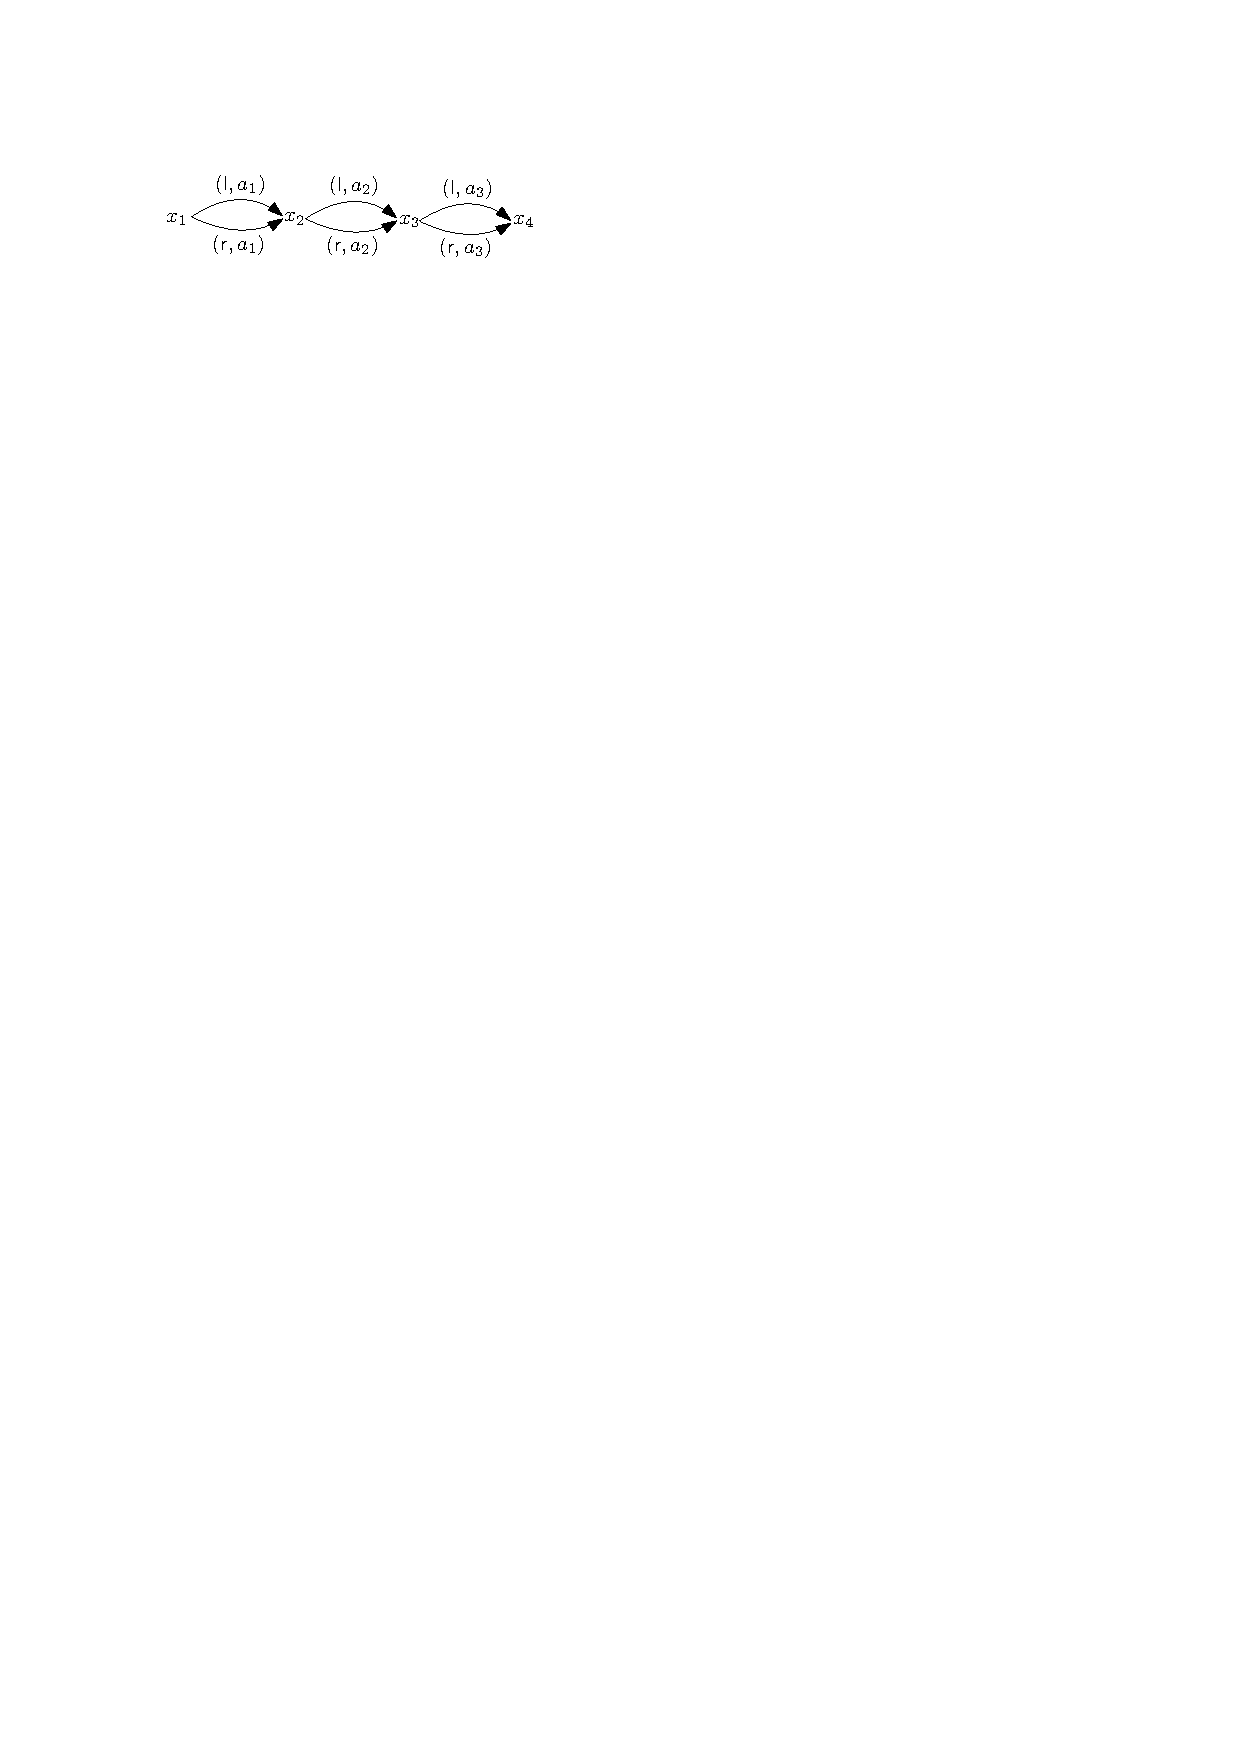
\includegraphics[scale=0.7]{dmdidx-example.pdf}
\end{center}
\caption{The diamond index  and the number of paths in $G_C$}\label{fig-dmdidx-exmp}
\end{figure}
\end{example}

In Section~\ref{sec:replaceallsl}--\ref{sec:replaceallre}, we will apply a refined analysis of the complexity of the decision procedures for proving Theorem~\ref{thm-main} and get the following results.

\begin{corollary}\label{cor-pspace}
The satisfiability problem is PSPACE-complete for the following fragments of $\strline[\replaceall]$:
\begin{itemize}
\item the single-letter case, plus the condition that the diamond indices of the dependency graphs are bounded by a constant $c$, 
%
\item the constant-string case, plus the condition that the $\rpleft$-lengths of the dependency graphs are bounded by a constant $c$, 

%
\item the regular-expression case, plus the condition that the $\rpleft$-lengths of the dependency graphs are at most $1$.
\end{itemize}
\end{corollary}

Corollary~\ref{cor-pspace} partially justifies our choice to present the decision procedures for the single-letter, constant-string, and regular-expression case separately. Intuitively, when the pattern parameters of $\replaceall$ terms become less restrictive, the decision procedures become more involved, and more constraints should be put on the dependency graphs in order to achieve the PSPACE upper bound. The PSPACE lower bound follows from the observation that the nonemptiness of the intersection of the regular expressions $e_1, \cdots, e_n$ over the alphabet $\{0,1\}$, which is a PSPACE-complete problem, can be reduced to the satisfiability of the formula $y = \replaceall((a b)^n, a, x) \wedge x \in (0+1)^\ast \wedge y \in e_1 \circ b  \circ \cdots \circ b \circ e_n$ (where $a, b \not \in \{0,1\}$), which belongs to all fragments in Corollary~\ref{cor-pspace}.\zhilin{Remark for the pspace lower bound, please check.}

%The proof of Theorem~\ref{thm-main} utilises a concept of dependency graphs defined below.



%Therefore,  in the following, without loss of generality, we assume that 
%in each $\strline[\replaceall]$ constraint $C=\varphi \wedge \psi$, the concatenation symbol $\concat$ does not occur in $\varphi$. 
 






\section{A decision procedure for $\pstrline[\replaceall]$} \label{sec:replaceallpure}

\subsection{Encode concatenation by replaceall}

We will transform a given constraint $\varphi$ into a constraint $\varphi'$ which is concatenation free. As the first step, we extend the original alphabet with two fresh letters $a,b$. 

For each $x=yz$, we introduce a new variable $x'$ and replace $x=yz$ by two new constraints 
$x'=\replaceall(ab, a, x)$ and $x=\replaceall(x', b, z)$. 

\begin{proposition}
	$\varphi$ and $\varphi'$ are equisatisfiable. 	
\end{proposition}

\subsection{The single-letter case}

We start with the single-letter special case, that is, given an $\pstrline[\replaceall]$ formula $C$, it holds that every term of the form $\replaceall(z, u, z')$ in $C$ satisfies that $u$ is a single letter.

We first introduce a concept of dependency graphs.

\begin{definition}[Dependency graph]
	Let $C= \varphi \wedge \psi$ be an $\pstrline[\replaceall]$ formula such that $\vars(\varphi) = \{x_1,\dots, x_m, y_1, \dots, y_n\}$, where $y_1,\dots, y_n$ are the source variables. Define the \emph{dependency graph} of $C$ as $G_C= (\vars(\varphi), E_C)$, such that for each $i \in [m]$, if $x_i = \replaceall(z, a_i, z')$, then $(x_i, (\rpleft, a_i), z) \in E_C$ and $(x_i, (\rpright, a_i), z') \in E_C$. A final (resp. initial) vertex in $G_C$ is a vertex in $G_C$ without successors (resp. predecessors). The edges labeled by $(\rpleft,a_i)$ and $(\rpright, a_i)$ are called the $\rpleft$-edges and $\rpright$-edges respectively. 
	%The $\rpleft$-length of a path $\pi$, denoted by $\rpleftlen(\pi)$, is the number of $\rpleft$-edges on $\pi$. A path of $G_C$ is a sequence $z_1 \ell_1 z_2 \dots \ell_{k-1} z_k$ such that for each $i \in [k-1]$, $(z_i, \ell_i, z_{i+1}) \in E_C$. A path is initial (resp. final) if the path starts from an initial vertex (resp. stops at a final vertex).
	% e the $\src$-nesting-depth of $z$ in $G_C$, denoted by $\srcnd_{G_C}(z)$,  as the maximum number of $\src$-edges in paths from source variables to $z$.
\end{definition}
Note that $G_C$ is a DAG where the out-degree of each vertex is two or zero. 


For each tuple of strings $\vec{v}=(v_1,\dots, v_n)$, if for each $j \in [n]$, $y_j$ is assigned with the string $v_j$, then for each vertex $z$ in $G_C$, the value of $z$, denoted by $\val_{\vec{v}}(z)$, is determined by the values of those source variables $y_j$ that are reachable from $z$, and can be computed in a bottom-up way. 

\smallskip


We will use the following running example to illustrate the decision procedure.
%\begin{example}
Consider the $\pstrline[\replaceall]$ formula $C=\varphi \wedge \psi$, whose dependency graph of $\varphi$ is illustrated in Fig.~\ref{fig-one-letter} and the regular constraint $\psi = \bigwedge \limits_{i \in [4]} x_i \in e_i \wedge \bigwedge \limits_{j \in [5]} y_j \in e'_j$. For $i \in [4]$ and $j \in [5]$, let us use $\cA_{x_i}$ and $\cA_{y_j}$ to denote the DFA corresponding to $e_i$ and $e'_j$ respectively.
\begin{figure}[htbp]
	\begin{center}
		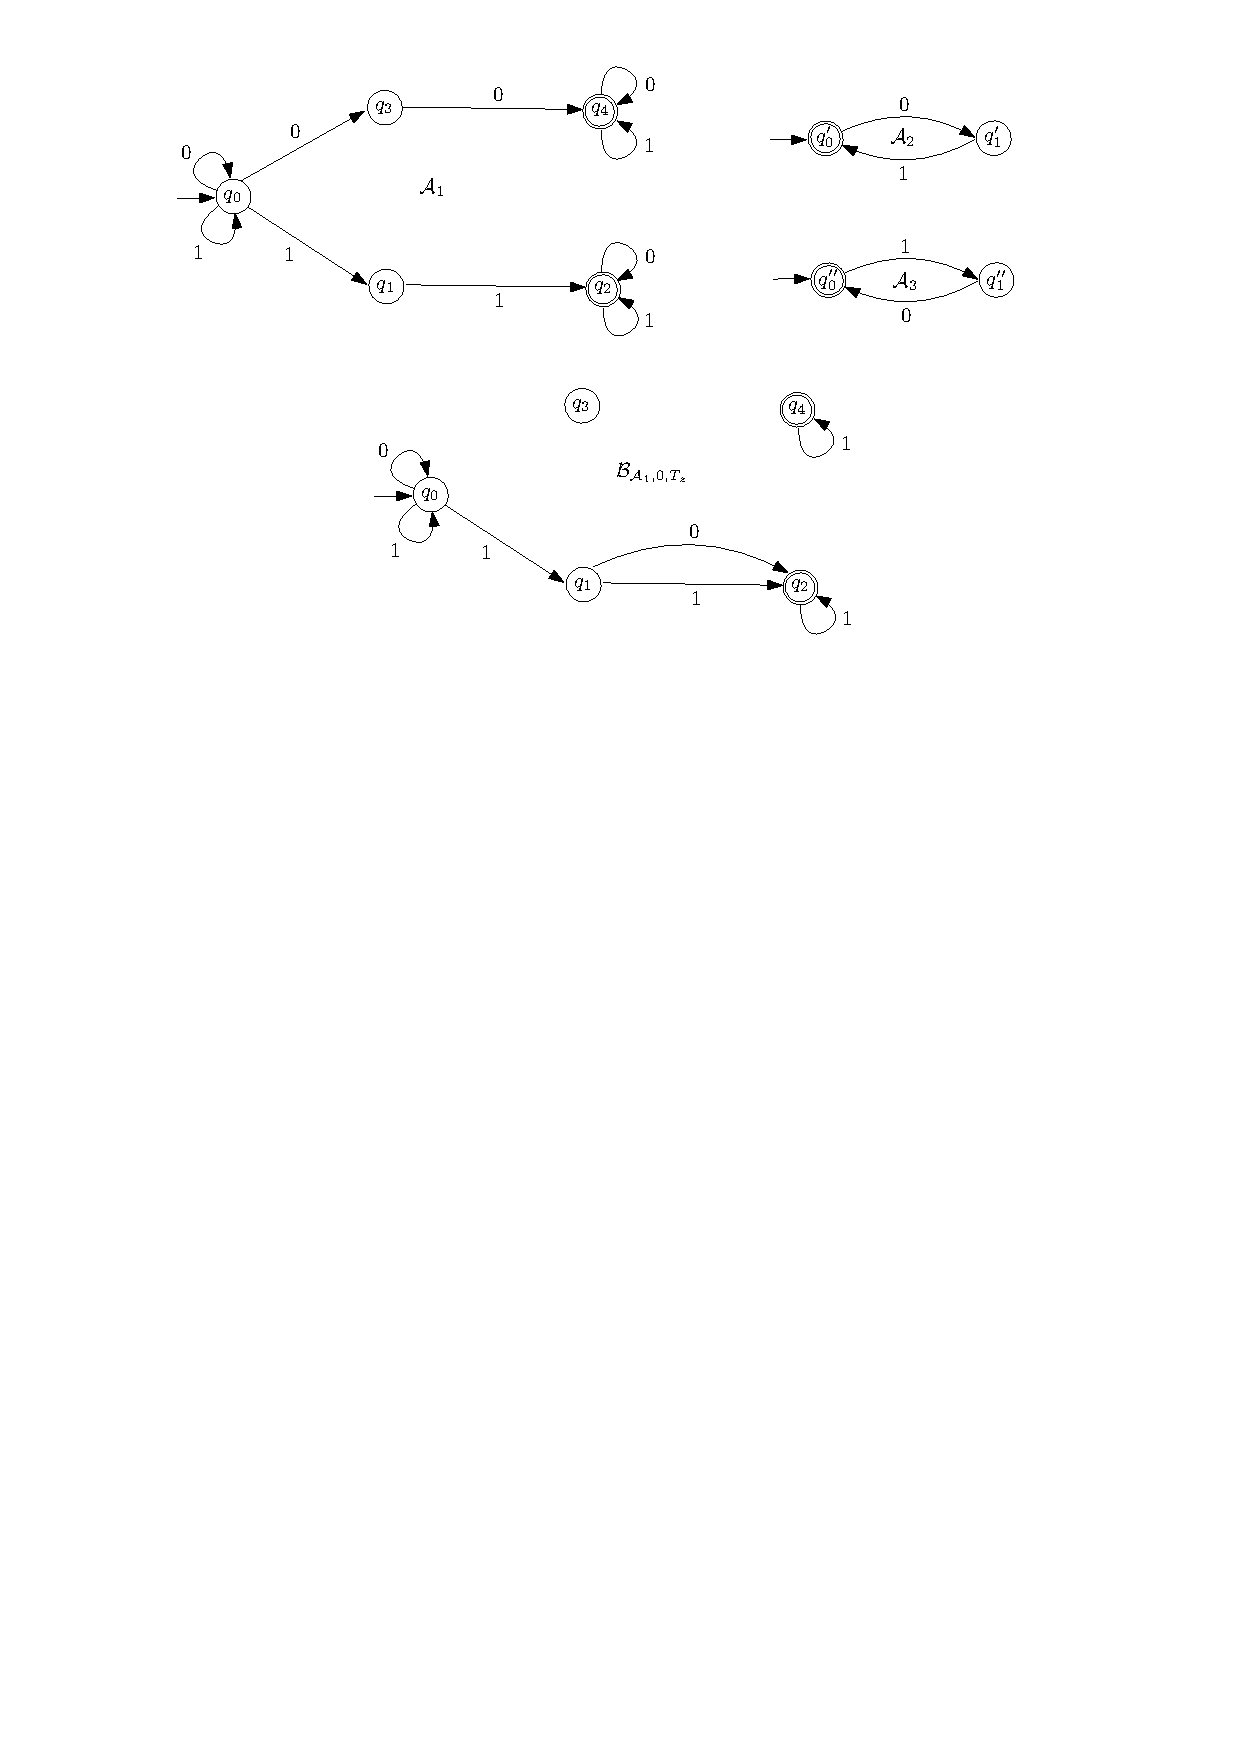
\includegraphics[scale=0.9]{single-letter-example.pdf}
	\end{center}
	\caption{The running example for the single-letter case}\label{fig-one-letter}
\end{figure}
%\end{example}
%



We will construct an NFA $\cA_C$ and reduce the satisfiability of $C=\varphi \wedge \psi$ to the nonemptiness of $\cA_C$. The inputs of $\cA_C$ are of the form $\triangleright \# v_1 \# \dots \# v_5\triangleleft$, where $v_1,\dots, v_5$ represent an assignment of the variables $y_1,\dots, y_5$. Intuitively, 
\begin{itemize}
	\item 
	$\cA_C$ checks whether for each $j \in [5]$, $v_j$ is accepted by $\cA_{y_j}$, 
	\item 
	in addition, let $\vec{v} = (v_1,\dots, v_5)$, then $\cA_C$ reads $\triangleright \# v_1 \# \dots \# v_5\triangleleft$, from left to right, and checks whether $\val_{\vec{v}}(x_i)$ is accepted by $\cA_{x_i}$, for each $i \in [4]$.
\end{itemize}

In the following, we will use the running example to give a more specific description of $\cA_C$. Let us introduce some additional notations.

\begin{definition}[$\cA$-context $\ctxt$ and $\red_\ctxt$]
	Suppose $\cA=(Q, \delta, q_0, F)$ is a DFA. Then an $\cA$-\emph{context} $\ctxt$  is a sequence $(a_1,f_1) \dots  (a_r, f_r)$ such that for each $i \in [r]$, $a_i \in \Sigma$ and $f_i$ is a function from $Q$ to $Q$. 
	For an $\cA$-context $\ctxt$, define the reduction of $\ctxt$, denoted by $\red_\ctxt$, as follows: $\red_\ctxt = (a_{i_1},f_{i_1})  \dots  (a_{i_s}, f_{i_s})$ such that for each $j \in [s]$, $a_{i_j} \not \in \{a_1,\dots, a_{i_j-1}\}$. 
\end{definition}
Intuitively, a reduction of $\ctxt$ is obtained by keeping the first occurrence of the letters and removing the other copies.

\begin{definition}[$\cB_{\cA, \ctxt}$]
	Suppose $\cA=(Q, \delta, q_0, F)$ is a DFA and $\ctxt$ is an $\cA$-context with $\red_\ctxt= (a_1,f_1) \dots  (a_r, f_r)$. We define a DFA $\cB_{\cA, \ctxt}$ as $(Q, \delta', q_0, F)$, where $\delta'$ comprises 1) all the tuples $(q, a', q') \in \delta$ with $a' \not \in \{a_1,\dots, a_r\}$, and 2) all the tuples $(q, a_i, f_i(q))$ such that $q \in Q$ and $i \in [r]$.
\end{definition}
Intuitively, over an input $w$, the DFA $\cB_{\cA, \ctxt}$ simulates the run of $\cA$ on $w$, with the following adaptation: let $\red_\ctxt= (a_1,f_1) \dots (a_r, f_r)$, then upon reading an occurrence of $a_i$, let $q$ be the current state, then after reading $a_i$, the state is changed to $f_i(q)$.

%\begin{definition}[Representatives of variables]
%For a variable $z \in \vars(\varphi)$,
%we define the representative of $z$, denoted by $\repr(z)$, as follows: If $z = y_j$ for some $j$, then $\repr(z) = y_j$, otherwise, let $\repr(z)$ be the unique source variable $y_j$ such that  there is a path from $x_i$ to $y_j$ where all edges are $\rpleft$-edges (The uniqueness of $y_j$ follows from the straight-line constraint). 
%\end{definition}

\begin{definition}[representative path]
	For a non-source variable $x_i \in \vars(\varphi)$, we define the representative path of $x_i$ as the unique path from $x_i$ to some source variable $y_j$ where all the edges are $\rpleft$-edges.  For a source variable $y_j$, define the representative path of $y_j$ be the empty path.
	%Note that for each non-source variable $x_i$, there is a unique source variable $y_j$ representing $x_i$. Let $\repr(x_i)$ denote this unique source variable $y_j$.
\end{definition}


We are ready to describe more details of the run of $\cA_C$ on $\triangleright \# v_1 \# \dots \# v_5\triangleleft$.

At first, for each path $\pi$ from a non-source variable $x_i$ to a source variable $y_j$,
%such that the label sequence of $\pi$ belongs to $\rpright^\ast \rpleft^\ast$, 
$\cA_C$ guesses a function $f_{\pi}$ on the state space of $\cA_{x_i}$, satisfying the following constraint: for each non-source variable $x_i$, let $\pi$ be the representative path of $x_i$, then $f_{\pi}(q_{0,x_i}) \in F_{x_i}$, where $q_{0, x_i}$ and $F_{x_i}$ are the initial state and the set of final states of $\cA_{x_i}$ respectively. 
% 
%Notice that for a given pair of variables $(x_i, y_j)$, let $N$ be the maximum length (number of edges) of the paths from $x_i$ to $y_j$, then there are at most $N+1$ distinct paths from $x_i$ to $y_j$ whose label sequences belong to $\rpright^\ast \rpleft^\ast$. Therefore, \emph{only polynomially many functions are guessed}.
%
%
Since $G_C$ is a tree, for simplicity, given a pair of distinct variables $z,z'$ such that $z'$ is reachable from $z$, we will use $\pi_{z,z'}$ to denote the unique path from $z$ to $z'$.  Let $\gfun$ denote the set of guessed functions.


Then $\cA_C$ verifies that the guessed functions satisfy some desired properties, when reading $\triangleright \# v_1 \# \dots \# v_5\triangleleft$.


For a path $\pi$, we define the context of $\pi$, denoted by $\ctxt_\pi$, inductively as follows: 
\begin{itemize}
	\item if $\pi$ is an empty path, then $\ctxt_\pi$ is the empty vector,
	% 
	\item otherwise, let the last edge of $\pi$ be from $z$ to $z'$ and $\pi'$ be the path obtained from $\pi$ by removing the last edge, then 
	\begin{itemize}
		\item if the last edge of $\pi$ is labeled by $(\rpright, a)$, then $\ctxt_\pi = \ctxt_{\pi'}$, 
		%
		\item if the last edge of $\pi$ is labeled by $(\rpleft, a)$,  let $z''$ be the destination vertex of the $\rpright$-edge out of $z$ and $\pi''$ denote the path obtained by concatenating $\pi'$, the $\rpright$-edge from $z$ to $z''$, and the representative path pf $z''$, then $\ctxt_\pi = (a, f_{\pi''}) \ctxt_{\pi'}$. 
		%
	\end{itemize}
\end{itemize}

For instance,  
$$
\begin{array}{l c l}
\ctxt_{\pi_{x_1, y_1}} &= & (a_3, f_{\pi_{x_1, y_2}}) \ctxt_{\pi_{x_1,x_3}} = (a_3, f_{\pi_{x_1, y_2}}) (a_2, f_{\pi_{x_1, y_3}}) \ctxt_{\pi_{x_1, x_2}}  \\
& = & (a_3, f_{\pi_{x_1, y_2}}) (a_2, f_{\pi_{x_1, y_3}}) (a_1, f_{\pi_{x_1, y_4}}).
\end{array}
$$

When reading $v_1$, $\cA_C$ does the following,
\begin{itemize}
	\item $\cA_C$ runs $\cA_{y_1}$ on $v_1$ to check that $v_1$ is accepted by $\cA_{y_1}$,
	%
	\item $\cA_C$ runs $\cB_{\cA_{x_3}, \ctxt_{\pi_{x_3,y_1}}}$ on $v_1$ to compute a function $f'_{\pi_{x_3,y_1}}$ on the state space of $\cA_{x_3}$ and checks $f'_{\pi_{x_3, y_1}} = f_{\pi_{x_3, y_1}}$,
	%
	\item  $\cA_C$ runs $\cB_{\cA_{x_2}, \ctxt_{\pi_{x_2,y_1}}}$ on $v_1$ to compute a function $f'_{\pi_{x_2,y_1}}$ on the state space of $\cA_{x_2}$ and checks $f'_{\pi_{x_2, y_1}} = f_{\pi_{x_2, y_1}}$, 
	
	% if $a_2 = a_3$, then $\cA_C$ runs $\cB_{\cA_{x_2}, a_3, f_{x_2, y_2}}$ on $v_1$ to compute a function $f'_{x_2,y_1}$  on the state space of $\cA_{x_2}$ and checks $f'_{x_2, y_1} = f_{x_2, y_1}$, otherwise, $\cA_C$ runs $\cB_{\cB_{\cA_{x_2}, a_3, f_{x_2, y_2}}, a_2, f_{x_2, y_3}}$ on $v_1$ to compute $f'_{x_2,y_1}$ and checks $f'_{x_2, y_1} = f_{x_2, y_1}$,
	%
	\item $\cA_C$ runs $\cB_{\cA_{x_1}, \ctxt_{\pi_{x_1,y_1}}}$ on $v_1$ to compute a function $f'_{\pi_{x_1,y_1}}$  on the state space of $\cA_{x_1}$ and checks $f'_{\pi_{x_1, y_1}} = f_{\pi_{x_1, y_1}}$.
\end{itemize}
We can also think the run of $\cA_C$ on $v_1$ as the run of $\cB_{y_1, \gfun}$ on $v_1$, where  $\cB_{y_1, \gfun}$ is the product automaton of $\cA_{y_1}$, $\cB_{\cA_{x_3}, \ctxt_{\pi_{x_3,y_1}}}$, $\cB_{\cA_{x_2}, \ctxt_{\pi_{x_2,y_1}}}$, and $\cB_{\cA_{x_1}, \ctxt_{\pi_{x_1,y_1}}}$. 

When reading $v_2$, $\cA_C$ does the following,
\begin{itemize}
	\item $\cA_C$ runs $\cA_{y_2}$ on $v_2$ to check that $v_2$ is accepted by $\cA_{y_2}$,
	%
	\item $\cA_C$ runs $ \cA_{x_3}$ on $v_2$ to compute a function $f'_{\pi_{x_3,y_2}}$ on the state space of $\cA_{x_3}$ and checks $f'_{\pi_{x_3,y_2}} = f_{\pi_{x_3, y_2}}$,
	%
	\item  $\cA_C$ runs $\cB_{\cA_{x_2}, \ctxt_{\pi_{x_2,y_2}}}$ on $v_2$ to compute a function $f'_{\pi_{x_2,y_2}}$ on the state space of $\cA_{x_2}$ and checks $f'_{\pi_{x_2,y_2}} = f_{\pi_{x_2, y_2}}$, 
	
	% if $a_2 = a_3$, then $\cA_C$ runs $\cB_{\cA_{x_2}, a_3, f_{x_2, y_2}}$ on $v_1$ to compute a function $f'_{x_2,y_1}$  on the state space of $\cA_{x_2}$ and checks $f'_{x_2, y_1} = f_{x_2, y_1}$, otherwise, $\cA_C$ runs $\cB_{\cB_{\cA_{x_2}, a_3, f_{x_2, y_2}}, a_2, f_{x_2, y_3}}$ on $v_1$ to compute $f'_{x_2,y_1}$ and checks $f'_{x_2, y_1} = f_{x_2, y_1}$,
	%
	\item $\cA_C$ runs $\cB_{\cA_{x_1}, \ctxt_{\pi_{x_1,y_2}}}$ on $v_2$ to compute a function $f'_{\pi_{x_1,y_2}}$  on the state space of $\cA_{x_1}$ and checks $f'_{\pi_{x_1, y_2}} = f_{\pi_{x_1, y_2}}$.
\end{itemize}
We can also think the run of $\cA_C$ on $v_2$ as the run of $\cB_{y_2, \gfun}$ on $v_2$, where  $\cB_{y_2, \gfun}$ is the product automaton of $\cA_{y_2}$, $ \cA_{x_3}$, $\cB_{\cA_{x_2}, \ctxt_{\pi_{x_2,y_2}}}$, and $\cB_{\cA_{x_1}, \ctxt_{\pi_{x_1,y_2}}}$. 


When reading $v_3$, $\cA_C$ does the following,
\begin{itemize}
	\item $\cA_C$ runs $\cA_{y_3}$ on $v_3$ to check that $v_3$ is accepted by $\cA_{y_3}$,
	%
	\item  $\cA_C$ runs $\cA_{x_2}$ on $v_3$ to compute a function $f'_{\pi_{x_2,y_3}}$ on the state space of $\cA_{x_2}$ and checks $f'_{\pi_{x_2,y_3}} = f_{\pi_{x_2, y_3}}$, 
	
	% if $a_2 = a_3$, then $\cA_C$ runs $\cB_{\cA_{x_2}, a_3, f_{x_2, y_2}}$ on $v_1$ to compute a function $f'_{x_2,y_1}$  on the state space of $\cA_{x_2}$ and checks $f'_{x_2, y_1} = f_{x_2, y_1}$, otherwise, $\cA_C$ runs $\cB_{\cB_{\cA_{x_2}, a_3, f_{x_2, y_2}}, a_2, f_{x_2, y_3}}$ on $v_1$ to compute $f'_{x_2,y_1}$ and checks $f'_{x_2, y_1} = f_{x_2, y_1}$,
	%
	\item $\cA_C$ runs $\cB_{\cA_{x_1}, \ctxt_{\pi_{x_1,y_3}}}$ on $v_3$ to compute a function $f'_{\pi_{x_1,y_3}}$  on the state space of $\cA_{x_1}$ and checks $f'_{\pi_{x_1, y_3}} = f_{\pi_{x_1, y_3}}$.
\end{itemize}
We can also think the run of $\cA_C$ on $v_3$ as the run of $\cB_{y_3, \gfun}$ on $v_3$, where  $\cB_{y_3, \gfun}$ is the product automaton of $\cA_{y_3}$, $ \cA_{x_2}$, and $\cB_{\cA_{x_1}, \ctxt_{\pi_{x_1,y_3}}}$. 


When reading $v_4$, $\cA_C$ does the following,
\begin{itemize}
	\item $\cA_C$ runs $\cA_{y_4}$ on $v_4$ to check that $v_4$ is accepted by $\cA_{y_4}$,
	%
	\item  $\cA_C$ runs $\cB_{\cA_{x_4}, \ctxt_{\pi_{x_4, y_4}}}$ on $v_4$ to compute a function $f'_{\pi_{x_4,y_4}}$ on the state space of $\cA_{x_4}$ and checks $f'_{\pi_{x_4,y_4}} = f_{\pi_{x_4, y_4}}$, 
	
	% if $a_2 = a_3$, then $\cA_C$ runs $\cB_{\cA_{x_2}, a_3, f_{x_2, y_2}}$ on $v_1$ to compute a function $f'_{x_2,y_1}$  on the state space of $\cA_{x_2}$ and checks $f'_{x_2, y_1} = f_{x_2, y_1}$, otherwise, $\cA_C$ runs $\cB_{\cB_{\cA_{x_2}, a_3, f_{x_2, y_2}}, a_2, f_{x_2, y_3}}$ on $v_1$ to compute $f'_{x_2,y_1}$ and checks $f'_{x_2, y_1} = f_{x_2, y_1}$,
	%
	\item $\cA_C$ runs $\cB_{\cA_{x_1}, \ctxt_{\pi_{x_1,y_4}}}$ on $v_4$ to compute a function $f'_{\pi_{x_1,y_4}}$  on the state space of $\cA_{x_1}$ and checks $f'_{\pi_{x_1, y_4}} = f_{\pi_{x_1, y_4}}$.
\end{itemize}
We can also think the run of $\cA_C$ on $v_4$ as the run of $\cB_{y_4, \gfun}$ on $v_3$, where  $\cB_{y_4, \gfun}$ is the product automaton of $\cA_{y_4}$, $\cB_{\cA_{x_4}, \ctxt_{\pi_{x_4, y_4}}}$, and $\cB_{\cA_{x_1}, \ctxt_{\pi_{x_1,y_4}}}$. 


When reading $v_5$, $\cA_C$ does the following,
\begin{itemize}
	\item $\cA_C$ runs $\cA_{y_5}$ on $v_5$ to check that $v_5$ is accepted by $\cA_{y_5}$,
	%
	\item  $\cA_C$ runs $\cA_{x_4}$ on $v_5$ to compute a function $f'_{\pi_{x_4,y_5}}$ on the state space of $\cA_{x_4}$ and checks $f'_{\pi_{x_4,y_5}} = f_{\pi_{x_4, y_5}}$, 
	%
	\item $\cA_C$ runs $\cB_{\cA_{x_1}, \ctxt_{\pi_{x_1,y_5}}}$ on $v_5$ to compute a function $f'_{\pi_{x_1,y_5}}$  on the state space of $\cA_{x_1}$ and checks $f'_{\pi_{x_1, y_5}} = f_{\pi_{x_1, y_5}}$.
\end{itemize}
We can also think the run of $\cA_C$ on $v_5$ as the run of $\cB_{y_5, \gfun}$ on $v_3$, where  $\cB_{y_5, \gfun}$ is the product automaton of $\cA_{y_5}$, $\cA_{x_4}$, and $\cB_{\cA_{x_1}, \ctxt_{\pi_{x_1,y_5}}}$. 

The nonemptiness of $\cA_C$ can be solved in exponential space as follows: 
\begin{description}
	\item [Step I.] For each path $\pi$ from a non-source variable $x_i$ to a source variable $y_j$, $\cA_C$ guesses a function $f_{\pi}$ on the state space of $\cA_{x_i}$.
	%
	\item  [Step II.] For each source variable $y_j$, guess an accepting run of $\cB_{y_j,\gfun}$.
\end{description}
Since at most exponentially many functions should be guessed, and each guessed function occupies polynomial space, it follows that the above procedure occupies only exponential space. If $G_C$ is a tree, then only polynomially many functions should be guessed and the above procedure occupies only polynomial space.

%\begin{theorem}
%The satisfiability of $\pstrline[\replaceall]$ is in EXPSPACE and PSPACE-complete for formulae whose dependency graphs trees.
%\end{theorem}

\subsection{The general case}

For the general case, we utilise the parsing-automata $\cA_u$ defined below.

Let $u \in \Sigma^+$ and $k=|u| \ge 2$.
Our goal is to construct an NFA $\cA_u=(Q_u, \delta_u, q_{0,u}, F_u)$ which parses a string $v \in \Sigma^\ast u \Sigma^\ast$ into $v_1 u v_2 u \dots v_l u v_{l+1}$ such that $v_j u[1] \dots u[k-1] \not \in \Sigma^\ast u \Sigma^\ast$ for each $1 \le j \le l$, in addition, $v_{l+1} \not \in \Sigma^\ast u \Sigma^\ast$. 
In order to check that a substring of $v$ is \emph{not} in $\Sigma^\ast u \Sigma^\ast$, we introduce a concept of $k$-window profiles w.r.t. $u$.


%If $u = \sigma$ for $\sigma \in \Sigma$, then $\cA_u=(Q_u, \delta_u, q_{0,u}, F_u)$, where $Q_u = \{(q_0, \bot), (q_0, \top) \}$, $\delta_u = \{(q_0, \bot) \xrightarrow{\sigma} (q_0, \top), (q_0, \bot) \xrightarrow{\Sigma \setminus \sigma} (q_0, \bot), (q_0, \top) \xrightarrow{ \sigma} (q_0, \top), (q_0, \top) \xrightarrow{\Sigma \setminus \sigma} (q_0, \bot)\}$, $q_{0,u} = (q_0, \bot)$, and $F_u = Q_u$.

%In the following, we assume that $|u| = k \ge 2$. Let $u = u_1 \dots u_k$, where each $u_i \in \Sigma$.

%We construct an NFA $\cA_u=(Q_u, \delta_u, q_{0,u}, F_u)$ which over a string $v$, parses $v \in \Sigma^\ast u \Sigma^\ast$ into $v_1 u v_2 u \dots v_l u v_{l+1}$ such that $v_j u_1 \dots u_{k-1} \not \in \Sigma^\ast u \Sigma^\ast$ for each $1 \le j \le l$, and $v_{l+1} \not \in \Sigma^\ast u \Sigma^\ast$. 
%Let $u = u_1\dots u_k$ such that $u_i \in \Sigma$ for each $i \in [k]$.  

A $k$-\emph{window profile $\vec{W}$ w.r.t. $u$} is an element of $\{\bot,\top\}^{k-1}$. Intuitively, in the position $i$ of a string $v$, $\vec{W}$ is an abstraction of the substring $v[i-k+2] \dots v[i]$ such that for each $j \in [k-1]$, $\vec{W}(j) = \top$ iff $v[i-j+1] \dots v[i] = u[1] \dots u[j]$. Let $\wprof_{u, k}$ denote the set of $k$-window profiles w.r.t. $u$. In particular, if $k = 1$, then $\wprof_{u, k} = \emptyset$. 

\zhilin{the following fact is noticed by Yan Chen.} 
Note that the number of $k$-window profiles w.r.t. $u$ is polynomial in the length of $u$. The arguments for this fact proceed as follows: For each profile $\vec{W}$, let $v$ be a string and $i$ be a position of $v$ such that for each $j \in [k-1]$, $\vec{W}(j) = \top$ iff $v[i-j+1] \dots v[i] = u[1] \dots u[j]$. Define ${\sf idx}_{\vec{W}}$ as the maximum index $j \in [k-1]$ such that $\vec{W}(j)=\top$. Then 
\begin{itemize}
	\item for each $j': j < j' < k$, $\vec{W}(j')=\bot$, 
	\item in addition, since $v[i-{\sf idx}_{\vec{W}}+1] \dots v[i] = u[1] \dots u[{\sf idx}_{\vec{W}}]$, the values of $\vec{W}(1),\dots, \vec{W}({\sf idx}_{\vec{W}})$ are completely determined by $u[1] \dots u[{\sf idx}_{\vec{W}}]$.
\end{itemize}
From the above arguments, we can  conclude that the number of $k$-window profile $\vec{W}$ w.r.t. $u$ is actually at most $k$.

\smallskip

The NFA $\cA_u$ is constructed as follows.
\begin{itemize}
	\item  $Q_u =\{q_0\} \cup \{(\search, \vec{W}) \mid \vec{W} \in \wprof_{u, k}\} \cup \{(\verify, j, \vec{W}) \mid j \in [k-1], \vec{W} \in \wprof_{u,k}\}$, where $q_0$ is a distinguished state whose purpose will become clear later on,  $\search$ and $\verify$ are used to denote whether $\cA_u$ is in the ``search''-mode to search the next occurrence of $u$, or in the ``verify'' mode to verify that the current position is a part of an occurrence of $u$.
	%
	\item $q_{0,u}=q_0$.
	
	\item $\delta_{u}$ comprises the following transitions,
	%guesses over each position, one of the following holds, the substring comprising the next $k$-symbols (including the current one) is $u$ or not.
	\begin{itemize}
		\item $q_0 \xrightarrow{\sigma} (\search, \vec{W})$, where $\vec{W}(1)=\top$ iff $\sigma = u[1]$, and for each $i: 2 \le i \le k-1$, $\vec{W}(i) = \bot$,
		%
		\item for each state $(\search, \vec{W})$ and $\sigma \in \Sigma$ such that $\vec{W}(k-1) = \bot$ or $\sigma \neq u[k]$,
		\begin{itemize}
			\item $(\search, \vec{W}) \xrightarrow{\sigma} (\search, \vec{W}')$, where $\vec{W}'(1) = \top$ iff $\sigma = u[1]$, and for each $i: 2 \le i \le k-1$, $\vec{W}'(i) =\top$ iff $\vec{W}({i-1}) = \top$ and $\sigma = u[i]$,
			%
			\item if $\sigma = u[1]$, then $(\search, \vec{W}) \xrightarrow{\sigma} (\verify, 1, \vec{W}')$,  where $\vec{W}'(1)=\top$,  and for each $i: 2 \le i \le k-1$, $\vec{W}'(i) =\top$ iff $\vec{W}({i-1}) = \top$ and $\sigma = u[i]$,
			%
		\end{itemize}
		%
		\item for each state $(\verify, i-1, \vec{W})$ such that
		\begin{itemize}
			\item $2 \le i \le k-1$,
			\item $\vec{W}(i-1)=\top$, $\sigma = u[i]$, and
			\item either $\vec{W}(k-1)=\bot$ or $\sigma \neq u[k]$, 
		\end{itemize}
		we have $(\verify, i-1, \vec{W}) \xrightarrow{\sigma} (\verify, i, \vec{W}')$, where for each $j: 2 \le j \le k-1$, $\vec{W}'(j) = \top$ iff $\vec{W}(j-1)=\top$ and $\sigma = u[j]$, 
		%
		\item for each state $(\verify, k-1, \vec{W})$ such that $\vec{W}(k-1)=\top$, we have $(\verify, k-1, \vec{W}) \xrightarrow{u[k]} q_0$.
		%where $\bot^k$ in $(\search, \bot^k)$ is used to \emph{reinitialise} the $k$-window profile w.r.t. $u$.
		%
	\end{itemize}
	Note that the constraint $\vec{W}(k-1) = \bot$ or $\sigma \neq u[k]$ is used to guarantee that when parsing a string $v$ into $v_1 u v_2 u \dots v_{l} u v_{l+1}$, $v_j u[1] \dots u[k-1] \not \in \Sigma^\ast u \Sigma^\ast$ for each $j \in [l]$, in addition, $v_{l+1} \not \in  \Sigma^\ast u \Sigma^\ast$.
	%
	\item $F_u=\{q_0\} \cup \{(\search, \vec{W}) \mid \vec{W} \in \wprof_{u, k} \} $. Note that the states $(\verify, j, \vec{W})$ are not final states, since when in these states, the verification of the next occurrence of $u$ has not yet been complete.
\end{itemize}
In an accepting run $r$ of $\cA_u$ on a string $v = v_1 u v_2 u \dots v_l u v_{l+1}$, the state sequence in the run is of the form 
$$q_0\ r_1\ q_0\ r_2\ q_0\ \dots\ r_l\ q_0\ r_{l+1}$$ 
such that  for each $j \in [l]$, $r_j \in (Q_{\search})^+ Q_{\verify, 1}  \dots  Q_{\verify, k-1}$, and $r_{l+1} \in (Q_{\search})^+$, where $Q_{\search}  = \{(\search, \vec{W}) \in \mid \vec{W} \in \wprof_{u,k}\}$, $Q_{\verify, 1} = \{(\verify, 1, \vec{W}) \mid \vec{W} \in \wprof_{u,k}\}, \dots, Q_{\verify, k-1}=\{(\verify, k-1, \vec{W}) \mid \vec{W} \in \wprof_{u, k}\}$. Intuitively, each occurence of $q_0$, except the first one, witnesses the \emph{first} occurrence of $u$ after its previous occurrence or starting from the beginning.

The NFA $\cA_u$ constructed above is \emph{unambiguous} in the sense that for each string $v \in \Sigma^+$, there is \emph{exactly one accepting run} of $\cA_u$ on $v$.

\begin{example}
	An example for $\cA_u$.
\end{example}

%Similarly to the single-letter case, we can define the dependency graph $G_C$. In addition, we can adapt $\dfs(z, z', a, f)$ into a procedure $\dfs(z, z', u, f)$, which integrates the automata $\cA_{u'}$ into the computation of the functions $f_{z', \cA_z}$, where $u,u'$ are constant strings occurring in the edge-labels in $G_C$.

\subsection{Extension to the case of regular expressions}

Let us consider the case that the second parameter of the $\replaceall$ function may be a regular expression. 
We will utilise the parsing-automaton $\cB_e$ for regular expressions $e$. 

We will use the leftmost and longest semantics for regular expression matching.

Let $e$ be a regular expression over $\Sigma$ and $\cA_e = (Q_e, \delta_e, q_{0,e}, F_e)$ be the DFA corresponding to $e$. Without loss of generality, we assume that $q_{0, e} \not \in F_e$ and there are no transitions going into $q_{0,e}$.
Our goal is to construct an NFA $\cB_e=(Q'_e, \delta'_e, q'_{0,e}, F'_e)$ which parses a string $v \in \Sigma^\ast e \Sigma^\ast$ into $v_1 u_1 v_2 u_2 \dots v_l u_l v_{l+1}$ such that 
\begin{itemize}
	\item for each $j \in [l]$, $u_j$ is the leftmost and longest matching of $e$ in $(v_1 u_1 \dots v_{j-1} u_{j-1})^{-1} v$,
	%
	%\item $v_j u_j[1] \dots u_j[|u_j|-1] \not \in \Sigma^\ast e \Sigma^\ast$ for each $1 \le j \le l$, in addition, $v_{l+1} \not \in \Sigma^\ast e \Sigma^\ast$,
	\item $v_{l+1} \not \in \Sigma^\ast e \Sigma^\ast$.
\end{itemize}
%
Intuitively, in order to search for the leftmost and longest matching of $e$, 
\begin{itemize}
	\item $\cB_e$ starts a new thread which runs $\cA_e$ in each position and keeps a vector of states of these threads, 
	%
	\item when a thread enters a final state, a matching of $e$ is found, $\cB_e$ nondeterministically guesses whether this matching is the longest matching, 
	%
	\item if $\cB_e$ makes the ``longest'' guessing, then $\cB_e$ forgets all the other threads, and continues running this thread to make sure that final states are not reached and the guessing is correct,
	%
	\item moreover, in order to keep the length of the vectors of states of threads \emph{bounded}, the following trick is applied: for two threads starting at the position $i$ and $j$ respectively such that $i < j$, if the current states of the two threads are the same, then the thread $j$ is removed.
\end{itemize}
%
Formally, 
\begin{itemize}
	\item the state set $Q'_e$ of $\cB_e$ comprises 
	\begin{itemize}
		\item the tuples $((q_{0,e}), \leftmost, S)$ such that $S \subseteq Q_e$,
		%
		\item $(\rho, \leftmost, S)$ such that  $\rho$ is a vector of \emph{pairwise distinct} states of $\cA_e$, $\rho \neq (q_{i,e})$, and $S \subseteq Q_e \setminus F_e$, 
		%
		% \item the tuples $(q_{0,e}, \longest, S)$ such that  $S \subseteq Q_e$,
		%
		\item the tuples $(q, \longest, S)$ such that $q \in Q_e$ and $S \subseteq Q_e \setminus F_e$;
	\end{itemize}
	%
	\item $q'_{0,e}= ((q_{0,e}), \leftmost, \emptyset)$,
	%
	\item $F'_{e}$ comprises the states of the form $(\rho, \leftmost, S) \in Q'_e$,
	%
	\item $\delta'_e$ comprises the following tuples: 
	\begin{itemize}
		%\item $((q_{0,e}, \leftmost, S), a, ((\delta_e(q_{0,e},a), q_{0,e}), \leftmost, \delta_e(S,a)))$, where $\delta_e(S,a) = \{\delta_e(q,a) \mid q \in S \}$,
		%
		\item suppose $\rho = q_1 \dots q_m$,  $a \in \Sigma$, $\delta_e(\rho, a) = \delta_e(q_1,a) \dots \delta_e(q_m, a)$ contains \emph{no} states from $F_e$, $\delta_e(S,a) = \{\delta_e(q,a) \mid q \in S \}$, and $\delta_e(S,a) \cap F_e = \emptyset$, then 
		$$((\rho, \leftmost, S), a, (\red(\delta_e(\rho,a) q_{0,e}), \leftmost, \delta_e(S,a))) \in \delta'_e,$$ 
		%
		\item suppose $\rho = q_1 \dots q_m$, $a \in \Sigma$, $\delta_e(\rho, a) = \delta_e(q_1,a) \dots \delta_e(q_m, a)$ contains at least one state from $F_e$, $i \in [m]$ is the smallest index such that $\delta_e(q_i, a) \in F_e$,   and $\delta_e(S,a) \cap F_e = \emptyset$, then 
		$$((\rho, \leftmost, S), a, (\delta_e(q_i, a), \longest, \delta_e(S,a))) \in  \delta'_e,$$ 
		%
		\item suppose $\rho = q_1 \dots q_m$, $a \in \Sigma$, $\delta_e(\rho, a) = \delta_e(q_1,a) \dots \delta_e(q_m, a)$, $\delta_e(\rho,a)$ contains at least one state from $F_e$, $i \in [m]$ is the smallest index such that $\delta_e(q_i, a) \in F_e$, and $\delta_e(S,a) \cap F_e = \emptyset$, then 
		$$((\rho, \leftmost, S), a, ((q_{0,e}), \leftmost, \delta_e(S,a) \cup \{\delta_e(q_i, a)\})) \in  \delta'_e,$$ 
		%
		\item suppose $\delta_e(S,a) \cap F_e = \emptyset$, then 
		$$((q, \longest, S), a, (\delta_e(q,a), \longest, \delta_e(S,a)) \in \delta'_e,$$
		%
		\item suppose $\delta_e(q,a) \in F_e$ and $\delta_e(S,a) \cap F_e = \emptyset$, then 
		$$((q, \longest, S), a, ((q_{0,e}), \leftmost, \delta_e(S,a) \cup \{\delta_e(q,a)\}) \in \delta'_e.$$
	\end{itemize}
\end{itemize}



%\subsection{A decision procedure for $\strline[\replaceall]$}




%!TEX root = popl2018.tex

\section{Undecidable extensions}

In this section, we extend the language $\strline[\replaceall]$ with integer and character constraints. The language will use two types of variables, str and int. 

We start by defining integer constraints, which expresses length or number of occurrences of symbols in words. 

\begin{definition}
	Each term is either 
	\begin{enumerate}
		\item an integer variable $n$;
		\item $|x|$ for a string variable;
		\item $|x|_a$ for $a\in \Sigma$
	\end{enumerate}
\end{definition}

Recall the Hilbert 10th problem, which is, for any given Diophantine equation (a polynomial equation with integer coefficients and a finite number of unknowns), to decide whether the equation has a solution with all unknowns taking integer values. It is easy to observe that given two polynomials with positive integral coefficients over the same set of variables $x_1, \cdots, x_n$, it is undecidable to check whether $f(x_1, \cdots, x_n)=g(x_1, \cdots, x_n)$ has a solution in natural numbers. 

\begin{theorem}
	The satisfiability problem for SL with length constraints is undecidable. 
\end{theorem}

\begin{proof}
	We shall reduce from the aforementioned version of the Hilbert tenth problem. For any polynomial with positive integral  $f(x_1, \cdots, x_n)$ where each coefficient is a positive 
\end{proof}

\subsection{Undecidability of character and length constraints}

Character constraints allow use to compare symbols from different strings. 

\begin{definition}
	An atomic character constraint over $\Sigma$ is an expression of the form $x[u]=y[v]$ where $x$ and $y$ are either a variable or a word in $\Sigma^*$, and $u$ and $v$ are either integer variables or constants positive integers. 
	
	A character constraint over $\Sigma$ is a Boolean combination of atomic character constraints over $\Sigma$. 
\end{definition}

Intuitively, $x[u]$ is interpreted as the $u$-th letter of $x$. 

We have the following simple observation:

\begin{lemma}
	For any two strings $x,y\in a^*\$$, $|x|=|y|$ iff $\exists n. x[n]=y[n]=\$$. 
\end{lemma}
\tl{I am not satisfied with this as the quantifier is used}

\paragraph{IndexOf}
One reason of introducing character constraints is, apart from the use of the JavaScript string method chatAt (which is used rather frequently in JavaScript according to the benchmark \cite{}), they can also be used to define IndexOf, which is the most standard usage of IndexOf method in practice. We consider the \emph{first-occurrence} semantics, i.e., (the first position in $x$ where $w$ occurs).
and the \emph{anywhere} semantics. 

We have the following observation: 
\begin{lemma}
	For any two strings $x,y$ over $\{a\}$, $x=y$ iff $1=IndexOf(x,y)=IndexOf(y,x)$.  
\end{lemma}

It follows that 
\begin{proposition}
	$\strline[\replaceall]$ extended with IndexOf is undecidable, regardless of the first-occurrence and the anywhere semantics. 
\end{proposition}

\subsection{Extensions with disequalities and IndexOf}
 
 %!TEX root = popl2018.tex

\section{Related work}\label{sec-rel}

 
In this section, we discuss some related work. We will classify our discussions into two main categories: (1) theoretical results in terms of decidability and complexity; (2) practical (but generally incomplete) approaches used in string solvers.  We shall emphasise work regarding $\replaceall$ functions as they are our main focus. 

\paragraph{Theoretical results}
We have discussed in Section \ref{sec:intro} works on string constraints with 
the theory of strings with concatenation. This research programme builds on
the question of solving satisfiability of \emph{word equations}, i.e., a
string equation $\alpha = \beta$ containing concatenation of string constants
and variables. Makanin showed decidability \cite{Makanin}, whose upper bound
was improved to PSPACE in \cite{P04} using a word compression technique. 
A simpler algorithm was in recent years proposed in \cite{J17} using
the recompression technique. The best lower bound for this problem is still NP,
and closing this complexity gap is a long-standing open problem. Decidability
(in fact, the PSPACE upper bound) can be retained in the presence of regular
constraints (e.g. see \cite{Schulz}). This can be extended to existential theory
of concatenation with regular constraints using the technique of \cite{buchi}.
The replace-all operator expressed by the concatenation operator alone. For 
this reason, our decidability of the fragment of $\strline[\replaceall]$ cannot
be derived from the results from the theory of concatenation alone.

%Our work is closely related to solving word equations, which are a conjunction of equations of $v=w$, where $v, w$ are concatenation of string constants and variables. The computational complexity of this problem remains unknown, with the best lower and upper bounds being NP and PSPACE respectively. Makanin %refuted a conjecture 
%showed, perhaps surprisingly, that the problem is decidable \cite{Makanin}, and %Plandowski's  on the decidability and complexity of satisfiability for word equations, i.e., 
%Plandowski explored an approach of compression and proposed a PSPACE algorithm \cite{P04}.  This is the best bound up to date, though a simpler PSPACE algorithm with smaller space requirement (nondeterministic $O(n \log n)$ space) was proposed by Jez \cite{J16}, based on compression. Very recently, Jez \cite{J17} further improves the complexity to (nondeterministic) $O(n )$, i.e.,  linear space. 

%The connection between compression and word equations was first observed by Plandowski and Rytter \cite{PR98}. %, who showed that a length-minimal solution of size N has a compressed representation
%of size poly(n, log N). 
\OMIT{
Essentially, the constraint language  $\strline[\replaceall]$ studied in this paper is word equations where the $\replaceall$ functions, which subsume the concatenation operation, are used. However, the additional straight-line restrictions are imposed.  
}

Regarding the extension with length constraints, it is still a long-standing
open problem whether word equations with length constraints is decidable, though
it is known that letter-counting (e.g. counting the number of occurrences of 0s
and 1s separately) yields undecidability \cite{buchi}. It was shown in
\cite{LB16} that the length constraints (in fact, letter-counting) can be
added to the subclass of $\strline[\replaceall]$ where the pattern/replacement 
are constants, while preserving decidability. In contrast, if we allow 
variables on the replacement strings of formulas in $\strline[\replaceall]$,
we can easily encode the Hilbert's 10th problem with length (integer) 
constraints. In fact, this undecidability holds even if we use the unary
alphabet $\Sigma = \{a\}$, and that the pattern string is
always fixed to the letter $a$.

%Solving word equation was an intriguing problem since the beginning of computer science, investigated
%initially due to its ties to Hilbert’s 10th problem. Initially it was conjectured that this
%problem is undecidable, which was disproved by Makanin [10]. At the beginning little attention
%was given to computational complexity of Makanin’s algorithm and the problem itself; these questions
%were reinvestigated in the ’90 [6, 18, 9], culminating in the EXPSPACE implementation of
%Makanin’s algorithm by Gutiérrez [5].


%\cite{J17}
%Word equations in linear space
%
%Word equations are an important problem on the intersection of formal languages and algebra. Given two sequences consisting of letters and variables we are to decide whether there is a substitution for the variables that turns this equation into true equality of strings. The computational complexity of this problem remains unknown, with the best lower and upper bounds being NP and PSPACE. Recently, a novel technique of recompression was applied to this problem, simplifying the known proofs and lowering the space complexity to (nondeterministic) O(n log n). In this paper we show that word equations are in nondeterministic linear space, thus the language of satisfiable word equations is context-sensitive. We use the known recompression-based algorithm and additionally employ Huffman coding for letters. The proof, however, uses analysis of how the fragments of the equation depend on each other as well as a new strategy for nondeterministic choices of the algorithm, which uses several new ideas to limit the space occupied by the letters.


\OMIT{
%A Decision Procedure for String Logic with Equations, Regular Membership and Length Constraints 
 Le \cite{L16} considered the satisfiability problem for string logic with word equations, regular membership and Presburger constraints over length functions. %The difficulty comes from multiple occurrences of string variables making state-of-the-art algorithms non-terminating. Our main contribution is to 
He showed that the satisfiability problem in a fragment where no string variable occurs more than twice in an equation is decidable. 
%In particular, he proposed a semi-decision procedure for arbitrary string formulae with word equations, regular membership and length functions, and showed that the algorithm always terminates for the aforementioned decidable fragment, with a complexity analysis. 
This work is largely distant from ours, as $\replaceall$ was not addressed. However, we mention that the fragment considered by Le allows Presburger constraints over length functions.
%The essence of our procedure is an algorithm to enumerate an equivalent set of solvable disjuncts for the formula. We further show that the algorithm always terminates for the aforementioned decidable fragment. Finally, we provide a complexity analysis of our decision procedure to prove that it runs, in the worst case, in factorial time.

%In \cite{BTV09} the authors discussed the problem of path feasibility for programs manipulating strings using a collection of standard string library functions. They prove results on the complexity of this problem, including its undecidability in the general case and decidability of some special cases. \tl{how would it connect to ours?}
}



The $\replaceall$ function can be seen as a special, yet expressive, string transformation function, aka string transducer. From this viewpoint, the closest work is~\cite{LB16}, which we discuss extensively in the introduction. Here, we discuss two further 
%the $\replaceall$ function is also related to two 
recent transducer models: streaming string transducers \cite{AC10} and symbolic transducers \cite{symbolic-transducer}. 

A streaming string transducer is a finite state machine where  a finite set of string variables are used to store the intermediate results for output. The $\replaceall(x, e, y)$ term can be modelled by an extension of streaming string transducers \emph{with parameters}, that is, a streaming string transducer which reads an input string (interpreted as the value of $x$), uses $y$ as a free string variable which is presumed to be read-only, and updates a string variable $z$, which stores the computation result, by a string term which may involve $y$. Nevertheless, to the best of our knowledge, this extension of streaming string transducers has not been investigated so far. 

Symbolic transducers are an extension of Mealy machine to infinite alphabets by using a variable $cur$ to represent the symbol in the current position, and replacing the input and output letters in transitions with unary predicates $\varphi(cur)$ and terms involving $cur$ respectively. Symbolic transducers can model $\replaceall$ functions \emph{when the third parameter is a constant}. Inspired by symbolic transducers, it is perhaps an interesting future work to consider an extension of the $\replaceall$ function by allowing predicates as patterns. %to sequences of numerical values. 
For instance, one may consider the term $\replaceall(x, cur \equiv 0 \bmod 2, y)$ which replaces every even number in $x$ with $y$. %This, however, is not addressed in the current paper. 

Finally, the $\replaceall$ function is related to Array Folds Logic introduced by Daca et al \cite{DHK16}. The authors considered an extension of the quantifier-free theory of integer arrays with counting. The main feature of the logic is the \emph{fold} terms, borrowed from the folding concept in functional programming languages. Intuitively, a fold term applies a function to every element of the array to compute an output. If strings are treated as arrays over a finite domain (the alphabet), the $\replaceall$ function can be seen as a fold term. Nevertheless, the $\replaceall$ function goes beyond the fold terms considered in \cite{DHK16}, since it outputs a string (an array), instead of an integer. Therefore, the results in \cite{DHK16} cannot be applied to our setting.

\paragraph{Practical Solvers}
There is a large amount of recent work on developing practical string solvers, Kaluza~\cite{Berkeley-JavaScript}, Hampi~\cite{HAMPI}, Z3-str~\cite{Z3-str}, CVC4~\cite{cvc4}, Stranger~\cite{YABI14}, Norn~\cite{Abdulla14}, S3 and S3P~\cite{S3,TCJ16}, and FAT~\cite{Abdulla17}.
Among them, only Stranger, S3, and S2P support $\replaceall$.  

%String solvers that support concatenations and the replace-all operator are available. \cite{BTV09,TCJ14,YABI14,S3}

%\cite{BTV09} considered an efficient finite model finding method for string constraints. They develop a two-tier finite model finding procedure. First, an integer abstraction of string constraints are passed to an SMT (Satisfiability Modulo Theories) solver. The abstraction is either unsatisfiable, or the solver produces a model that fixes lengths of enough strings to reduce the entire problem to be finite domain. The resulting fixed-length string constraints are then solved in a second phase. 

%We implemented the procedure in a symbolic execution framework, report on the encouraging results and discuss directions for improving the method further.


In the Stranger tool, %Verifying string manipulating programs is a crucial problem in computer security. String operations are used extensively within web applications to manipulate user input, and their erroneous use is the most common cause of security vulnerabilities in web applications. We 
an automata-based approach was provided for symbolic analysis of PHP programs, where two different semantics $\replaceall$ were considered, namely, the leftmost and longest matching as well as the leftmost and shortest matching. Nevertheless, they focused on the abstraction-interpretation based analysis of PHP programs and provided an \emph{over-approximation} of all the possible values of the string variables at each program point. Therefore, their string constraint solving algorithm is \emph{not} an exact decision procedure. In contrast, we provided a decision procedure for the straight-line fragment with the rather general $\replaceall$ function, where the pattern parameter can be arbitrary regular expressions and the replacement parameter can be variables. In the latter case,  we consider the leftmost and longest semantics mainly for simplicity, and the decision procedure can be adapted to the leftmost and shortest semantics easily.

%%%%%%%%%%%%%%%%%%%%%%%%%%%%%%%%%%%%%%%%%%
%%%%%%%%%%%%%%%%%%%%%%%%%%%%%%%%%%%%%%%%%%
\hide{
 For the string operations, the authors focus on two common ones: concatenation and replacement. The latter is close to---but not the same as---the $\replaceall$ function considered in this paper. However, in this paper, Yu et al provided   an \emph{over-approximation} of more %restricted replace 
commonly used semantics, i.e., the longest match and first match semantics. 
%
%\cite{SMV12} translating regular expression matching into transducer. 
%
They use deterministic finite automata (DFAs) to represent possible values of string variables. Using forward reachability analysis we compute an over-approximation of all possible values that string variables can take at each program point. They also implemented Stranger, an automata-based string analysis tool, with experiments. In general, this is essentially an abstract interpretation based approach.  In comparison, our algorithm is also automata-based, but we work on a semantics of $\replaceall$, but not its approximation. \tl{more need to be said here}
}
%%%%%%%%%%%%%%%%%%%%%%%%%%%%%%%%%%%%%%%%%%
%%%%%%%%%%%%%%%%%%%%%%%%%%%%%%%%%%%%%%%%%%

%Intersecting these with a given attack pattern yields the potential attack strings if the program is vulnerable. Based on the presented techniques, we have implemented Stranger, an automata-based string analysis tool for detecting string-related security vulnerabilities in PHP applications. We evaluated Stranger on several open-source Web applications including one with 350,000+ lines of code. Stranger is able to detect known/unknown vulnerabilities, and, after inserting proper sanitization routines, prove the absence of vulnerabilities with respect to given attack patterns.

 
The S3 and S3P tools also support the $\replaceall$ function, where some
progressive searching strategies were provided to deal with the non-termination
problem brought out by the recursively defined string operations (of which the
$\replaceall$ function is a special case). Nevertheless, the solvers are 
incomplete as reasoning about unbounded strings defined recursively is in 
general an undecidable problem.


%, the authors present S3 (which stands for Symbolic String Solver), a new symbolic string solver.
%The constraint language covers all the main string operations including the replace-all function. The authors 
%provided algorithms which make use of a symbolic representation so that membership in a set defined by a regular expression can be encoded as string equations. 

%To amplify this point, let us now state some statistics from a comprehensive
%study of practical JavaScript applications [28]. Constraints
%arising from the applications have an average (per benchmark
%query) of 63 JavaScript string operations, while the remaining
%are boolean, logical and arithmetic constraints. The largest fraction
%are for operations like indexOf, length (78%). A significant
%fraction of the operations, including substring (5%), replace
%(8%), and split, match (1%). Of the match, split and
%replace operations, 31% are based on regular expressions. Operations
%such as replace and split give rise to new strings
%from the original ones, thereby giving rise to constraints involving
%multiple string variables.



%. The algorithm first makes use of a symbolic representation
%so that membership in a set defined by a regular expression
%can be encoded as string equations. Secondly, there is a constraint based
%generation of instances from these symbolic expressions so
%that the total number of instances can be limited. 
%
%We evaluate S3 on a well-known set of practical benchmarks, demonstrating both
%its robustness (more definitive answers) and its efficiency (about 20
%times faster) against the state-of-the-art.



\hide{
%Progressive Reasoning over Recursively-Defined Strings
\cite{TCJ16} 
Trinh et al considered %the problem of reasoning over an expressive constraint language for unbounded strings. 
%In particular, they considered 
recursively defined string functions, a very expressive way to define functions manipulating strings. This includes a recursive definition of the replace-all function considered in this paper\footnote{\cite{TCJ16} used the notation \textbf{replace}}. The authors argue that ``the difficulty comes from ``recursively defined" functions such as replace, making state-of-the-art algorithms non-terminating." They proposed a progressive search algorithm, %to not only mitigate the problem of non-terminating reasoning but also guide the search towards a “minimal solution” when the input formula is in fact satisfiable. We have 
implemented within the state-of-the-art Z3 framework, with experimental evaluations. The algorithm is genetic and  applicable to all recursively defined string functions, but it is doomed to be incomplete as reasoning about unbounded strings defined recursively is in general an undecidable problem.   

The focus of our work is on the fundamental issue of decidability, and this is complementary to the work. Our result may be considered a completeness guarantee for existing string solver. 
}

%Importantly, we have enabled conflict clause learning for string theory so that our solver can be used effectively in the setting of program verification. Finally, our experimental evaluation shows leadership in a large benchmark suite, and a first deployment for another benchmark suite which requires reasoning about string formulas of a class that has not been solved before.



%===========================================================
%
%\subsection*{Other related work}
 



%Symbolic Finite State Transducers:
%Algorithms and Applications

%
%Finite automata and finite transducers are used in a wide
%range of applications in software engineering, from regular
%expressions to specification languages. We extend these
%classic objects with symbolic alphabets represented as parametric
%theories. Admitting potentially infinite alphabets
%makes this representation strictly more general and succinct
%than classical finite transducers and automata over strings.
%Despite this, the main operations, including composition,
%checking that a transducer is single-valued, and equivalence
%checking for single-valued symbolic finite transducers are
%effective given a decision procedure for the background theory.
%We provide novel algorithms for these operations and
%extend composition to symbolic transducers augmented with
%registers. Our base algorithms are unusual in that they are
%nonconstructive, therefore, we also supply a separate model
%generation algorithm that can quickly find counterexamples
%in the case two symbolic finite transducers are not
%equivalent. The algorithms give rise to a complete decidable
%algebra of symbolic transducers. Unlike previous work, we
%do not need any syntactic restriction of the formulas on the
%transitions, only a decision procedure. In practice we leverage
%recent advances in satisfiability modulo theory (SMT)
%solvers. We demonstrate our techniques on four case studies,
%covering a wide range of applications. Our techniques
%can synthesize string pre-images in excess of 8, 000 bytes
%in roughly a minute, and we find that our new encodings
%significantly outperform previous techniques in succinctness
%and speed of analysis
% 

 
  \section{Conclusion}

%% Acknowledgments
%\begin{acks}                            %% acks environment is optional
                                        %% contents suppressed with 'anonymous'
  %% Commands \grantsponsor{<sponsorID>}{<name>}{<url>} and
  %% \grantnum[<url>]{<sponsorID>}{<number>} should be used to
  %% acknowledge financial support and will be used by metadata
  %% extraction tools.
%  This material is based upon work supported by the
%  \grantsponsor{GS100000001}{National Science
%    Foundation}{http://dx.doi.org/10.13039/100000001} under Grant
%  No.~\grantnum{GS100000001}{nnnnnnn} and Grant
%  No.~\grantnum{GS100000001}{mmmmmmm}.  Any opinions, findings, and
%  conclusions or recommendations expressed in this material are those
%  of the author and do not necessarily reflect the views of the
%  National Science Foundation.
%\end{acks}


%% Bibliography
%\bibliography{bibfile}
\bibliography{string}

%% Appendix
\appendix
\section{Appendix}

 

\end{document}
